\subsection{Large-Batch, Memory-Efficient, and Parameter-Free Optimizers}
\paragraph{LAMB (Layer-wise Adaptive Moments optimizer for Batch training).}
\begin{figure}[H]
\centering
\fitfigure{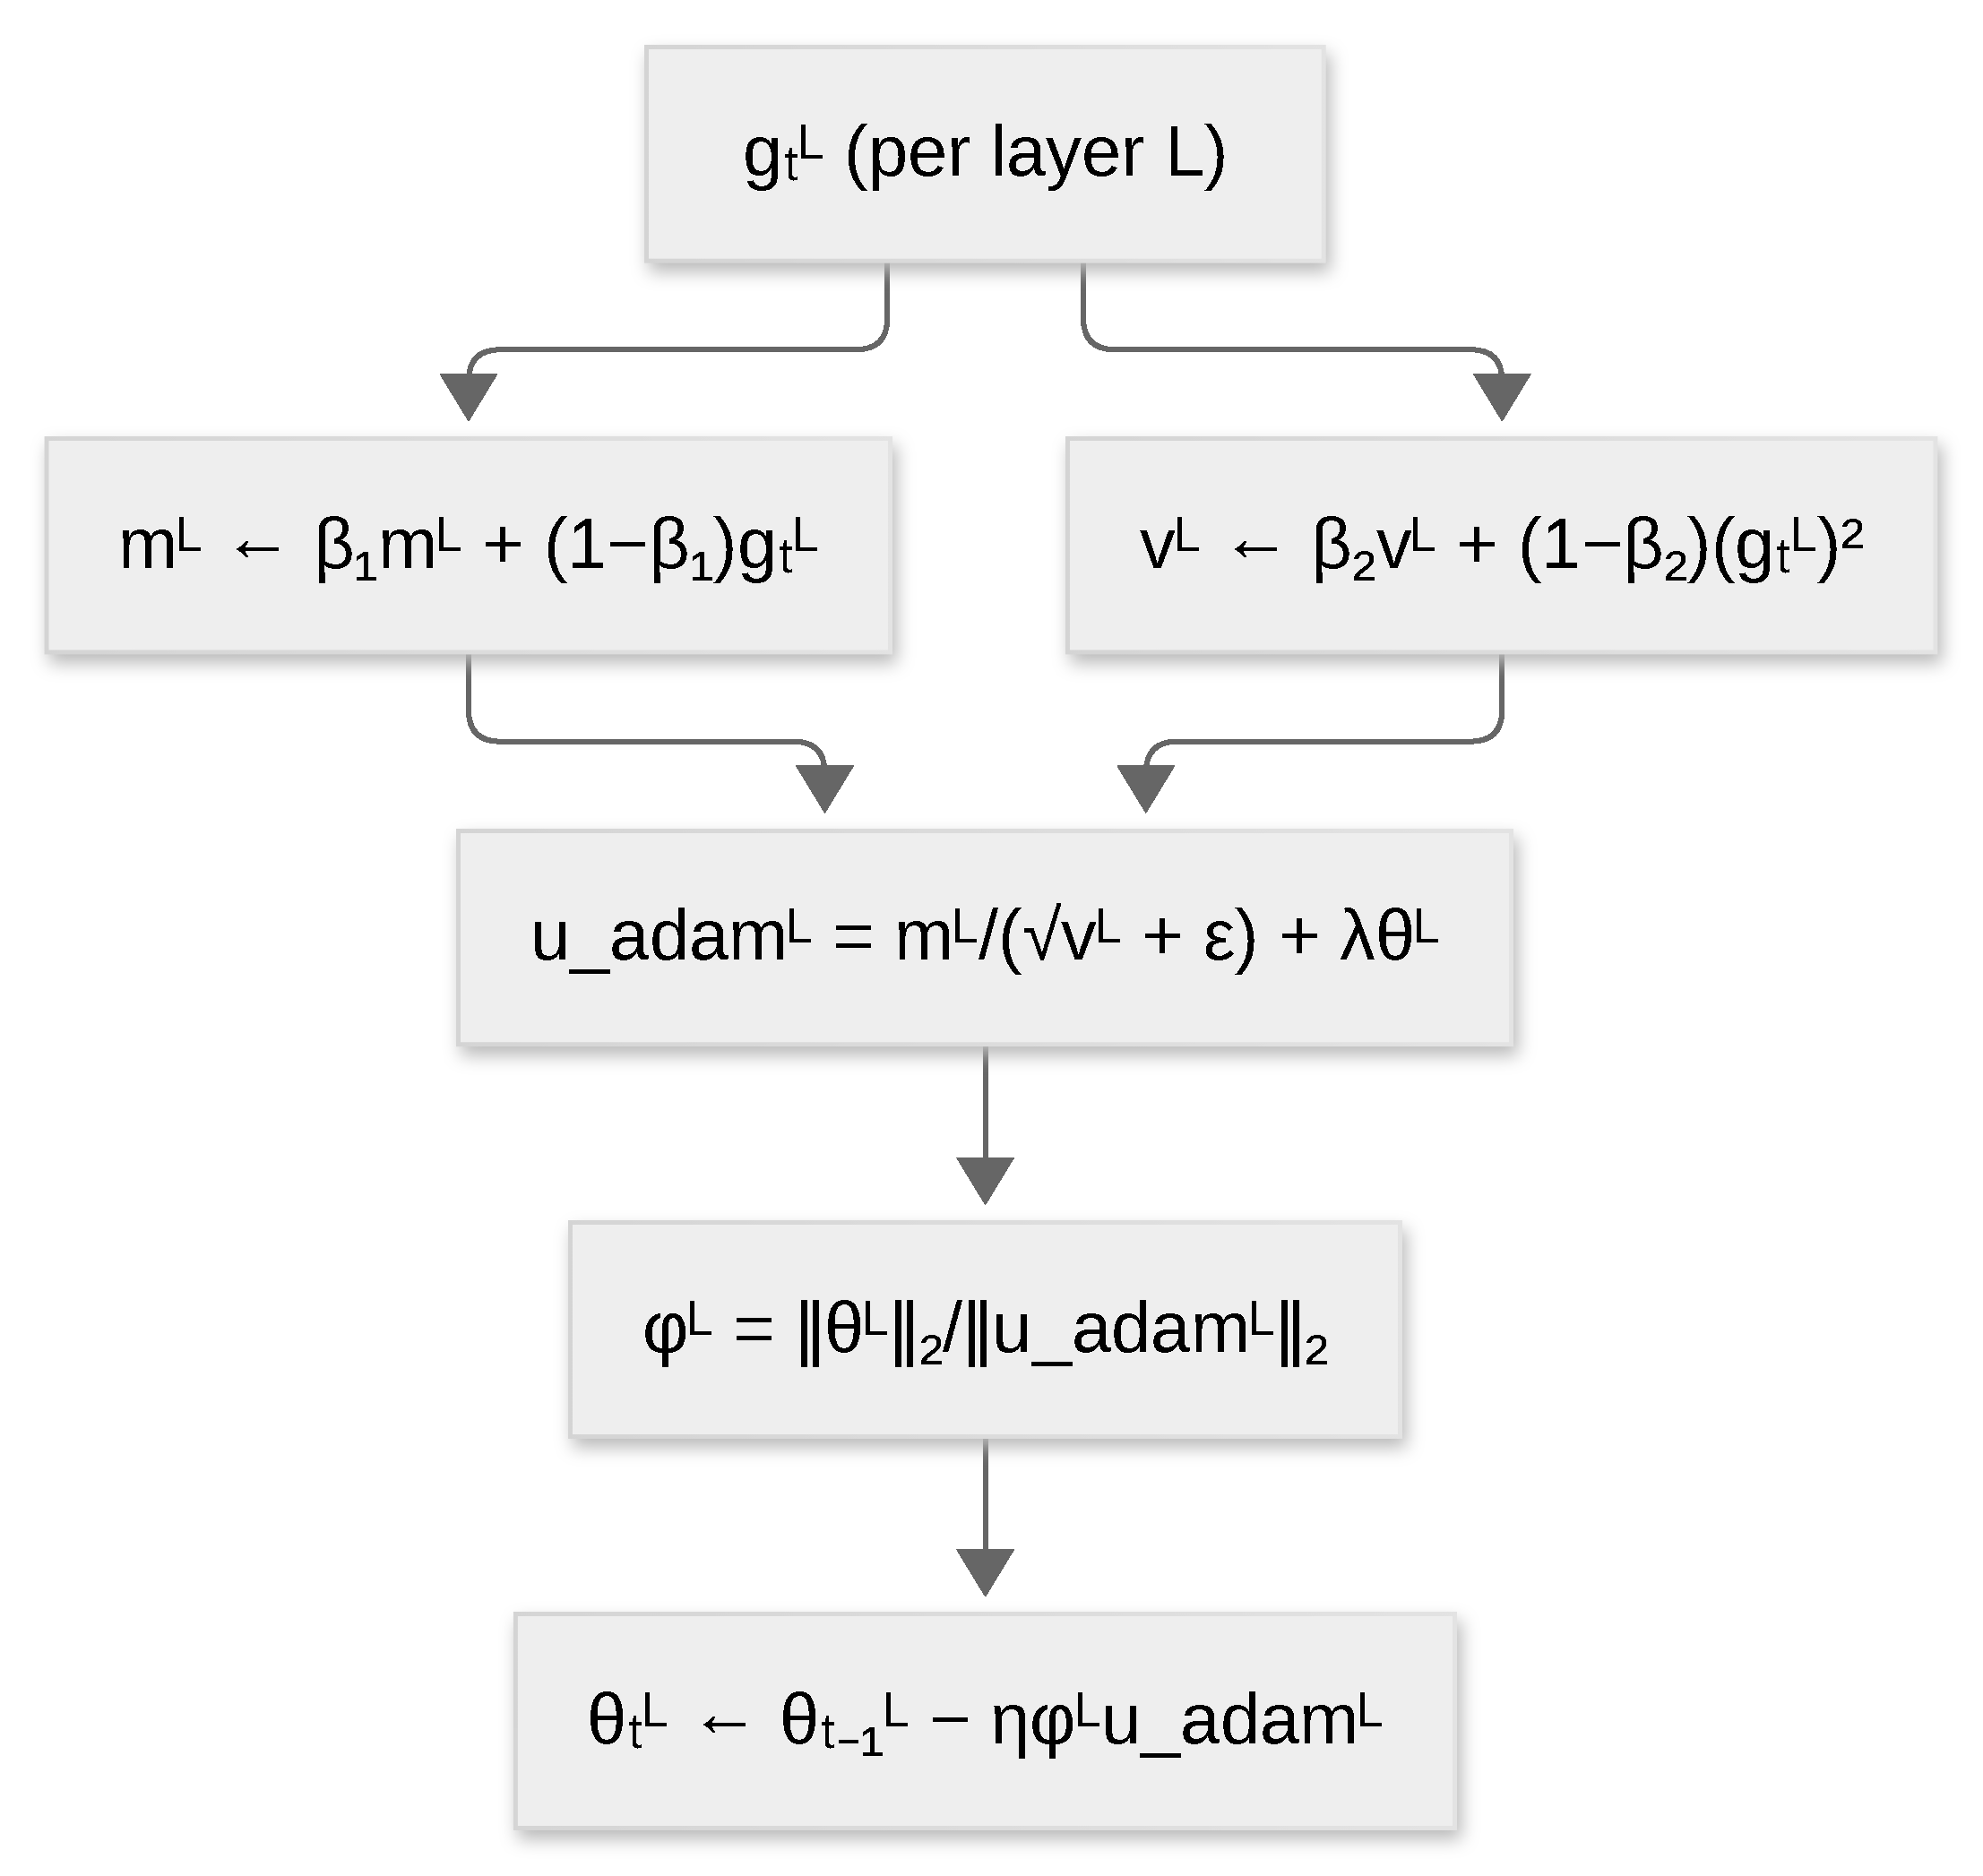
\includegraphics{figures/optimizers/lamb.pdf}}
\caption{Step flow of LAMB: per-layer Adam step rescaled by the trust ratio between weight and update norms.}
\label{fig:opt-lamb}
\end{figure}
LAMB extends Adam with \textbf{layer-wise adaptive rate scaling} (inspired by LARS), enabling stable training with extreme batch sizes (e.g., 64K on BERT):
\begin{align}
m_t^L &= \beta_1 m_{t-1}^L + (1-\beta_1)g_t^L \quad\text{(layer-wise first moment)} \\
v_t^L &= \beta_2 v_{t-1}^L + (1-\beta_2)(g_t^L)^2 \\
u_{\text{adam}}^L &= \frac{m_t^L}{\sqrt{v_t^L}+\epsilon} + \lambda\theta_{t-1}^L \quad\text{(base adaptive step with decay)} \\
\phi^L &= \frac{\|\theta_{t-1}^L\|_2}{\|u_{\text{adam}}^L\|_2} \quad\text{(trust ratio: layer normalization)} \\
\theta_t^L &= \theta_{t-1}^L - \eta \cdot \phi^L \cdot u_{\text{adam}}^L
\end{align}
The \textbf{trust ratio} $\phi^L = \|\theta^L\|_2 / \|u_{\text{adam}}^L\|_2$ normalizes the effective update step relative to weight magnitude. In very large batches, stochastic gradient noise can exceed signal, destabilizing layer-wise learning rates. By scaling updates proportionally to weight norms, LAMB ensures relative changes rather than absolute ones, preventing small confident updates in large vectors from dominating.

\begin{algorithm}[H]
\caption{LAMB (Layer-wise Adaptive Moments optimizer for Batch training)}
\label{alg:lamb}
\begin{algorithmic}[1]
\Require Initial parameters $\theta_0$, learning rate $\eta$, $\beta_1, \beta_2$, weight decay $\lambda$
\Ensure Updated parameters $\theta_T$
\State Initialize: For each layer $L$: $m^L \gets 0$, $v^L \gets 0$
\For{$t = 1, 2, \ldots, T$}
    \For{each layer $L$}
        \State $g_t^L \gets \nabla f(\theta_t^L)$
        \State $m^L \gets \beta_1 m^L + (1-\beta_1) g_t^L$
        \State $v^L \gets \beta_2 v^L + (1-\beta_2) (g_t^L)^2$
        \State Base Adam: $u_{\text{adam}}^L \gets m^L / (\sqrt{v^L} + \epsilon)$
        \If{weight\_decay $> 0$}
            \State $u_{\text{adam}}^L \gets u_{\text{adam}}^L + \lambda \theta_{t-1}^L$
        \EndIf
        \State Trust ratio: $\phi^L \gets \|\theta_{t-1}^L\|_2 / \|u_{\text{adam}}^L\|_2$ if both nonzero, else $1$
        \State $\theta_t^L \gets \theta_{t-1}^L - \eta \phi^L u_{\text{adam}}^L$
    \EndFor
\EndFor
\Return $\theta_T$
\end{algorithmic}
\end{algorithm}

\paragraph{Cons.}
\begin{itemize}[leftmargin=*]
\item Layer-wise norm bookkeeping and trust-ratio computation add per-step overhead.
\item The trust ratio is unstable when layer or update norms are close to zero.
\end{itemize}

\paragraph{Pros.}
\begin{itemize}[leftmargin=*]
\item Enables stable training with extreme batch sizes (e.g., 64K on BERT).
\item Preserves small-batch generalization benefits while scaling the batch.
\end{itemize}

\paragraph{Schedule-Free AdamW.}
\begin{figure}[H]
\centering
\fitfigure{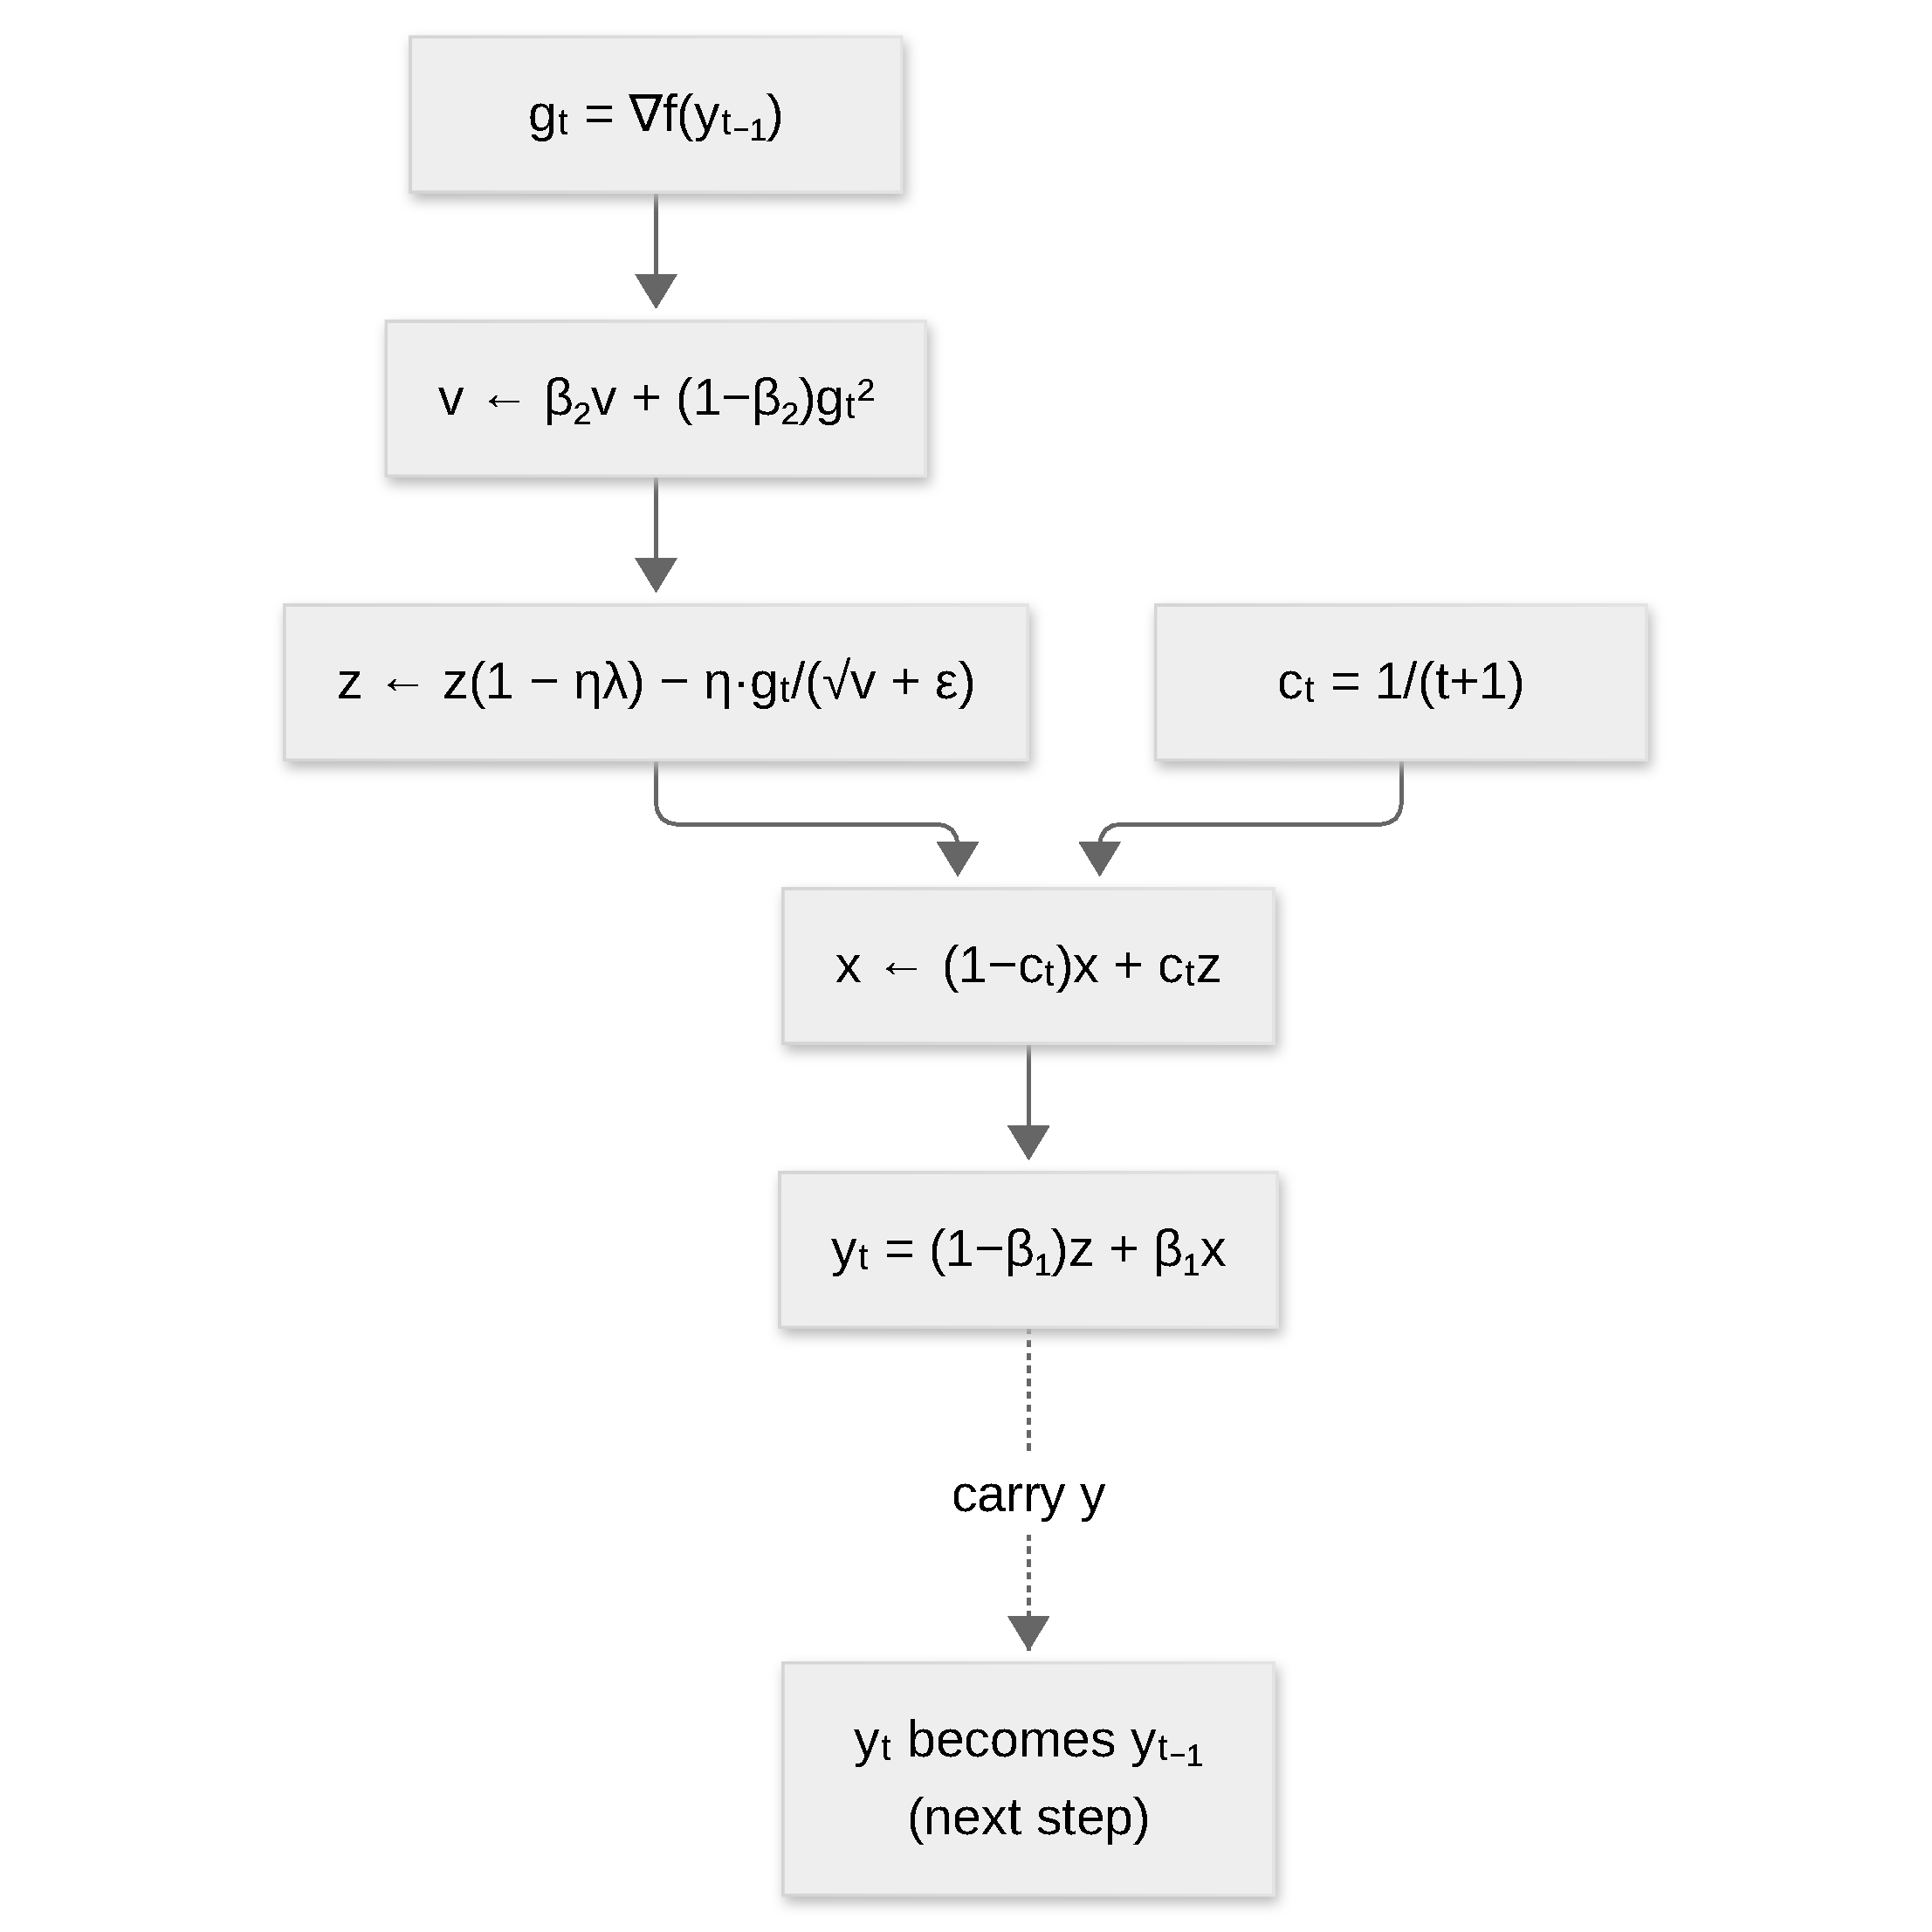
\includegraphics{figures/optimizers/schedulefree.pdf}}
\caption{Step flow of Schedule-Free AdamW: exploration stream $z$, iterate average $x$, and interpolation point $y$, with implicit $1/(t+1)$ averaging.}
\label{fig:opt-schedulefree}
\end{figure}
Schedule-free methods remove explicit scheduler design from the optimization recipe. The algorithm maintains two parameter streams: $z_t$ (exploration) and $x_t$ (smooth average):
\begin{align}
v_t &= \beta_2 v_{t-1} + (1-\beta_2)g_t^2 \quad\text{(variance)} \\
z_t &= z_{t-1}(1-\eta\lambda) - \eta\frac{g_t}{\sqrt{v_t}+\epsilon} \quad\text{(adaptive step with decay)} \\
c_t &= \frac{1}{t+1} \quad\text{(averaging coefficient, decreases over time)} \\
x_t &= (1-c_t)x_{t-1} + c_t z_t \quad\text{(iterate averaging)} \\
y_t &= (1-\beta)z_t + \beta x_t \quad\text{(interpolation for evaluation point)}
\end{align}
The averaging coefficient $c_t = 1/(t+1)$ implements an implicit learning-rate schedule without explicitly specifying total steps $T$. This framework unifies scheduling and iterate averaging: the algorithm explores via $z_t$ while accumulating stable direction via $x_t$. The evaluation point $y_t$ (used for gradient computation) interpolates between exploration and stability.

\begin{algorithm}[H]
\caption{Schedule-Free AdamW}
\label{alg:schedulefree}
\begin{algorithmic}[1]
\Require Initial parameters $\theta_0$, learning rate $\eta$ (fixed), $\beta_1, \beta_2$, weight decay $\lambda$
\Ensure Updated parameters $\theta_T$ or averaging $x_T$
\State Initialize: $z \gets \theta_0$ (exploration), $x \gets \theta_0$ (average), $v \gets 0$, $t \gets 0$
\For{$t = 1, 2, \ldots, T$}
    \State $g_t \gets \nabla f(y_{t-1})$ (gradient at interpolation point)
    \State $v \gets \beta_2 v + (1-\beta_2) g_t^2$ \Comment{Variance}
    \State Weight decay on $z$: $z \gets z(1 - \eta\lambda)$
    \State $z \gets z - \eta g_t / (\sqrt{v} + \epsilon)$ \Comment{Adaptive step on raw}
    \State $c_t \gets 1 / (t+1)$ \Comment{Averaging coefficient}
    \State $x \gets (1-c_t) x + c_t z$ \Comment{Iterate averaging}
    \State $y_t \gets (1-\beta_1) z + \beta_1 x$ \Comment{Interpolation for next eval}
\EndFor
\Return $x_T$ or $y_T$
\end{algorithmic}
\end{algorithm}

\paragraph{Cons.}
\begin{itemize}[leftmargin=*]
\item Maintains two parameter streams ($z$ and $x$) and requires explicit handling of the evaluation point.
\item Behavior departs from scheduled baselines, which complicates comparisons.
\end{itemize}

\paragraph{Pros.}
\begin{itemize}[leftmargin=*]
\item Removes the explicit learning-rate schedule and its total-step hyperparameter.
\item State-of-the-art convergence across convex optimization, large-scale deep learning, and reinforcement learning.
\end{itemize}

\paragraph{Adafactor.}
\begin{figure}[H]
\centering
\fitfigure{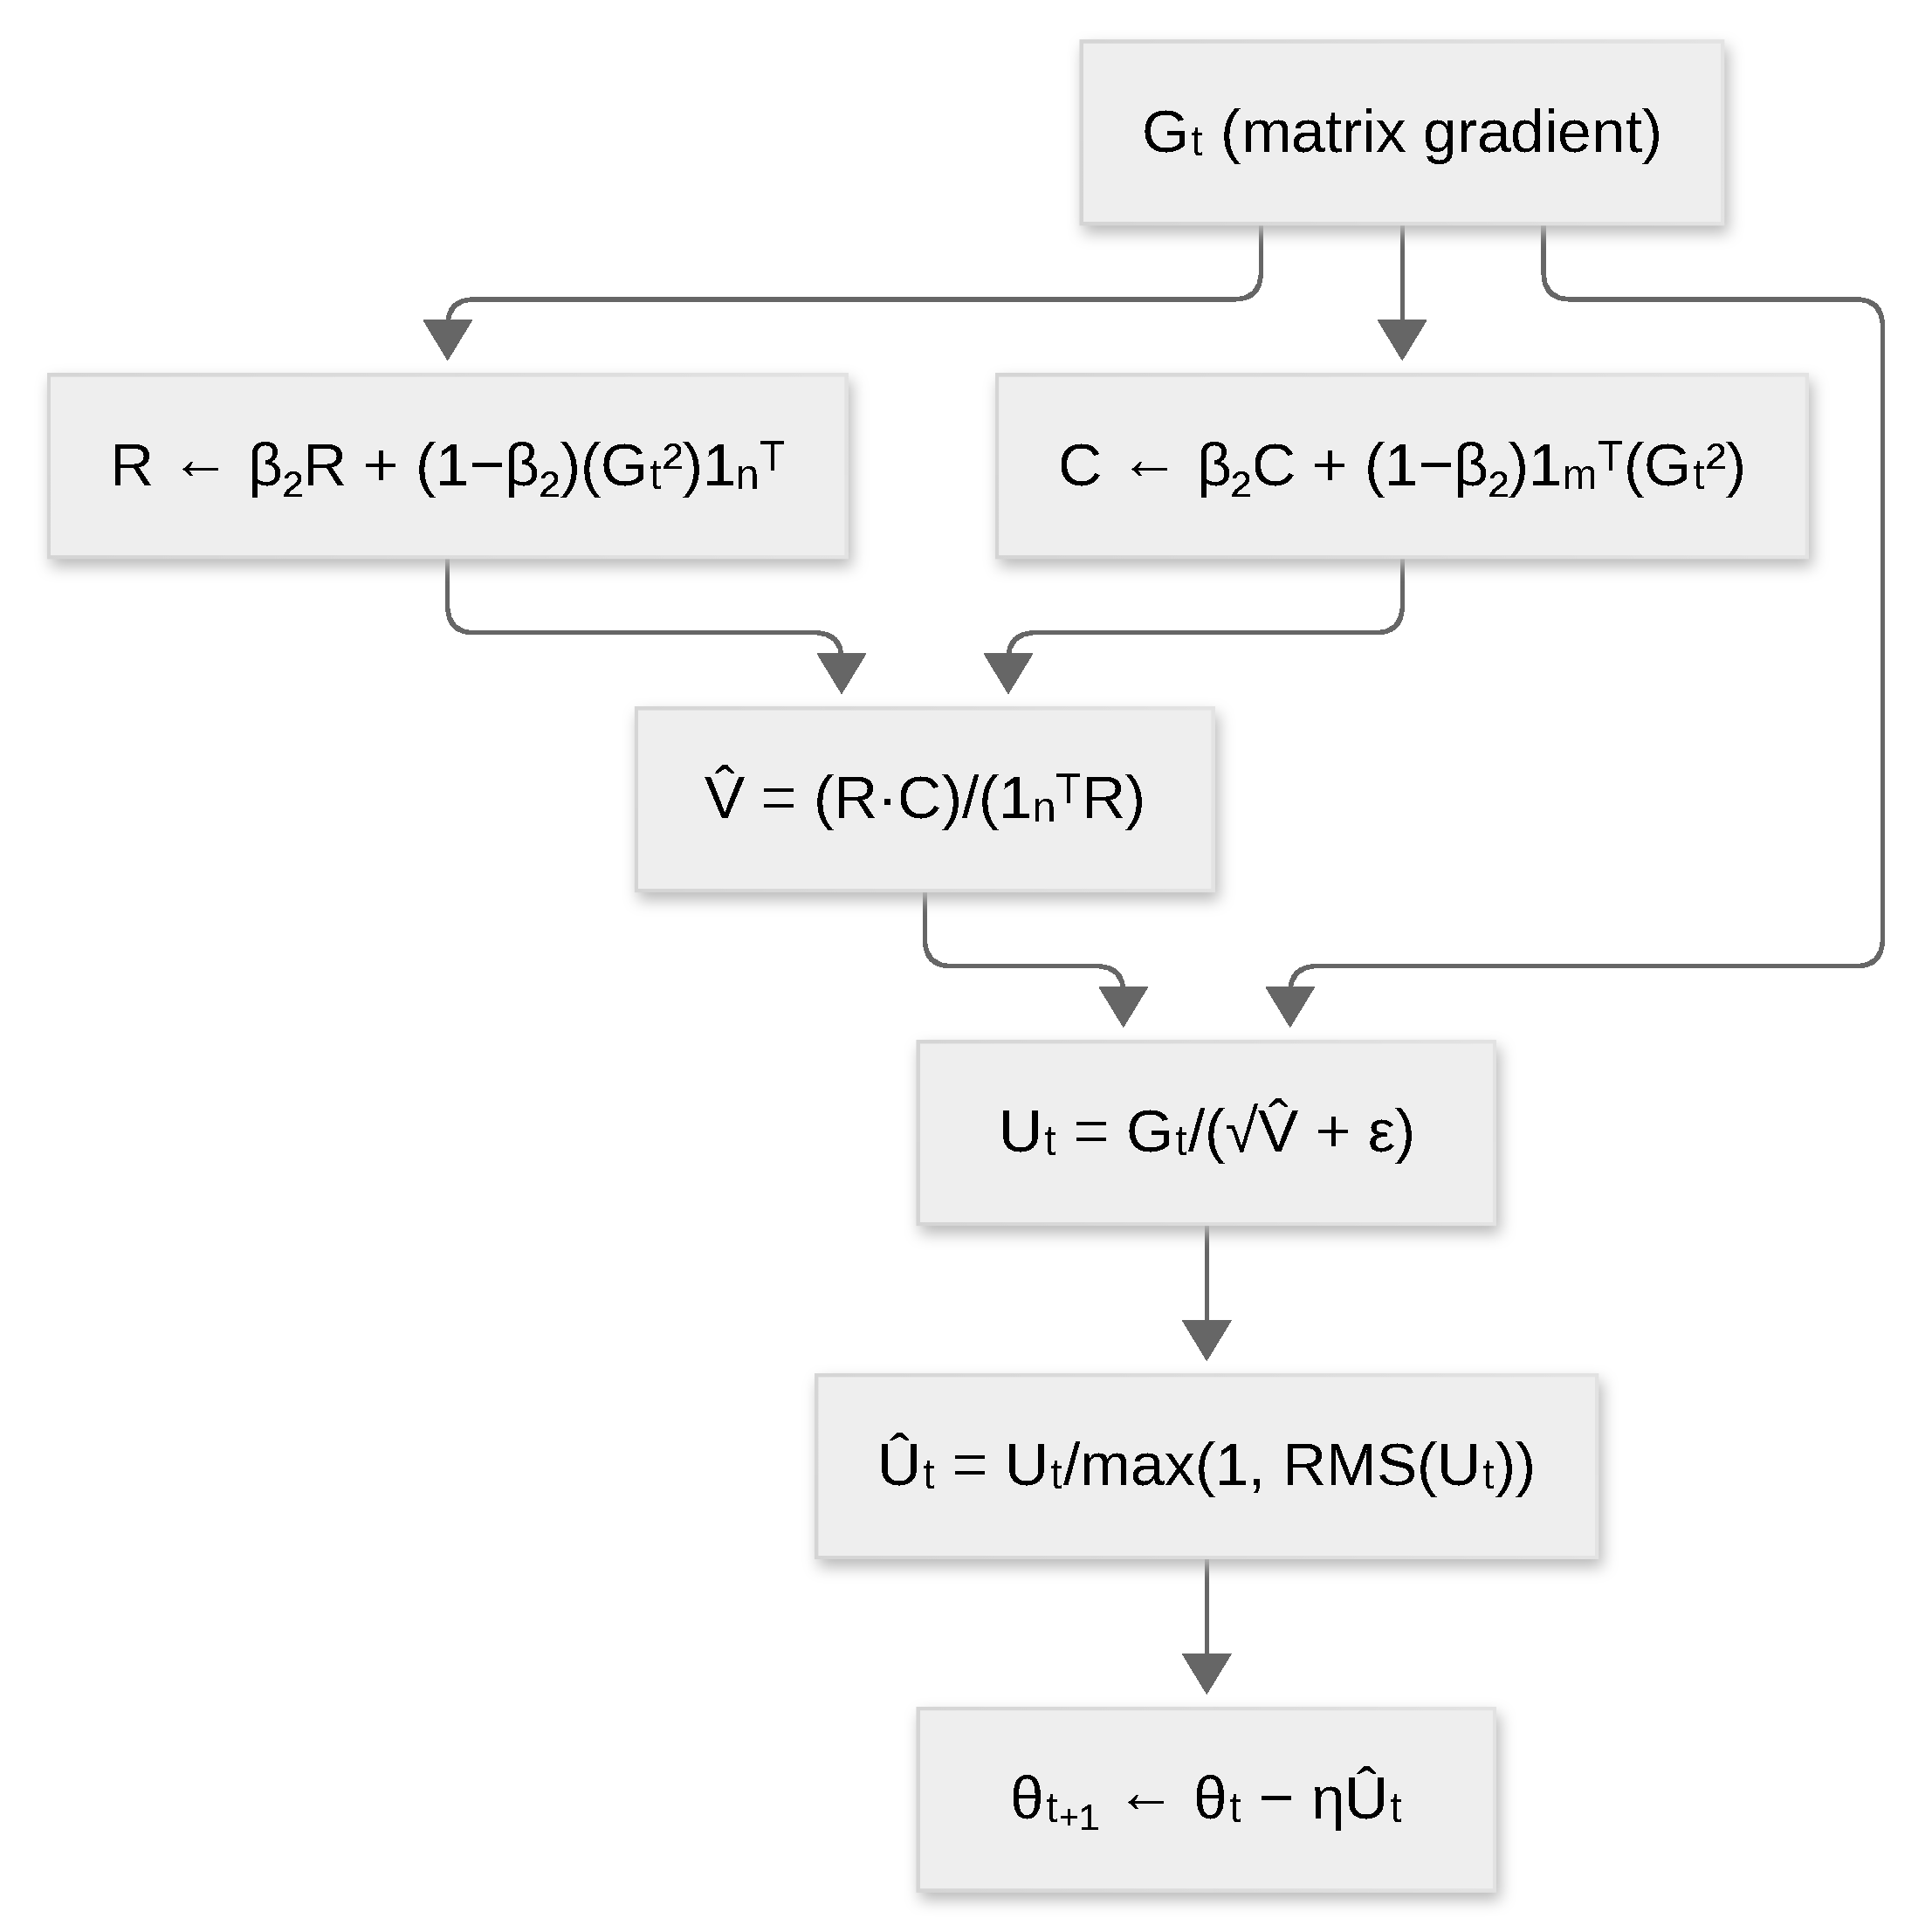
\includegraphics{figures/optimizers/adafactor.pdf}}
\caption{Step flow of Adafactor: factorized row/column second-moment accumulators, outer-product variance reconstruction, and RMS clipping.}
\label{fig:opt-adafactor}
\end{figure}
Adafactor reduces optimizer memory by \textbf{factorizing} second-moment statistics for matrix-shaped parameters, storing only row and column accumulators rather than dense variance states. For a gradient matrix $G_t \in \mathbb{R}^{m \times n}$:
\begin{align}
R_t &= \beta_2 R_{t-1} + (1-\beta_2)(G_t^2) \mathbf{1}_n^T \quad\text{(row variance)} \\
C_t &= \beta_2 C_{t-1} + (1-\beta_2) \mathbf{1}_m^\top (G_t^2) \quad\text{(column variance)} \\
\hat{V}_t &= \frac{R_t C_t}{\mathbf{1}_n^\top R_t} \quad\text{(reconstructed variance via outer product)} \\
U_t &= \frac{G_t}{\sqrt{\hat{V}_t}+\epsilon} \quad\text{(normalized adaptive step)} \\
\hat{U}_t &= \frac{U_t}{\max(1, \text{RMS}(U_t))} \quad\text{(stability clipping)}
\end{align}

\begin{algorithm}[H]
\caption{Adafactor (Factorized Second-Moment Statistics)}
\label{alg:adafactor}
\begin{algorithmic}[1]
\Require Gradient matrix $G_t \in \mathbb{R}^{m \times n}$, learning rate $\eta$, $\beta_2 \approx 0.999$
\Ensure Updated parameters $\theta_T$
\State Initialize: Row accumulators $R \gets \epsilon \mathbf{1}^T_m$, Column $C \gets \epsilon \mathbf{1}_n$
\For{$t = 1, 2, \ldots, T$}
    \State $G_t \gets \nabla f(\theta_t)$ (matrix gradient)
    \State $R \gets \beta_2 R + (1-\beta_2) (G_t^2) \mathbf{1}_n^T$ \Comment{Row inner products}
    \State $C \gets \beta_2 C + (1-\beta_2) \mathbf{1}_m^\top (G_t^2)$ \Comment{Column inner products}
    \State Reconstructed variance: $\hat{V} \gets (R \cdot C) / (\mathbf{1}_n^\top R)$ \Comment{Via outer product}
    \State Normalized adaptive step: $U_t \gets G_t / (\sqrt{\hat{V}} + \epsilon)$
    \State Per-row RMS clipping: $\hat{U}_t \gets U_t / \max(1, \text{RMS}(U_t))$
    \State $\theta_{t+1} \gets \theta_t - \eta \hat{U}_t$
\EndFor
\Return $\theta_T$
\end{algorithmic}
\end{algorithm}

\paragraph{Cons.}
\begin{itemize}[leftmargin=*]
\item Factorized variance is an approximation and can be unstable on some tasks.
\item Reduced optimization expressiveness relative to full Adam.
\end{itemize}

\paragraph{Pros.}
\begin{itemize}[leftmargin=*]
\item Memory drops from $O(n_{\text{params}})$ to $O(\sqrt{n_{\text{params}}})$ for matrix parameters.
\item Most attractive when VRAM is dominated by optimizer state rather than activations.
\end{itemize}

\paragraph{GaLore (Gradient Low-Rank Projection).}
\begin{figure}[H]
\centering
\fitfigure{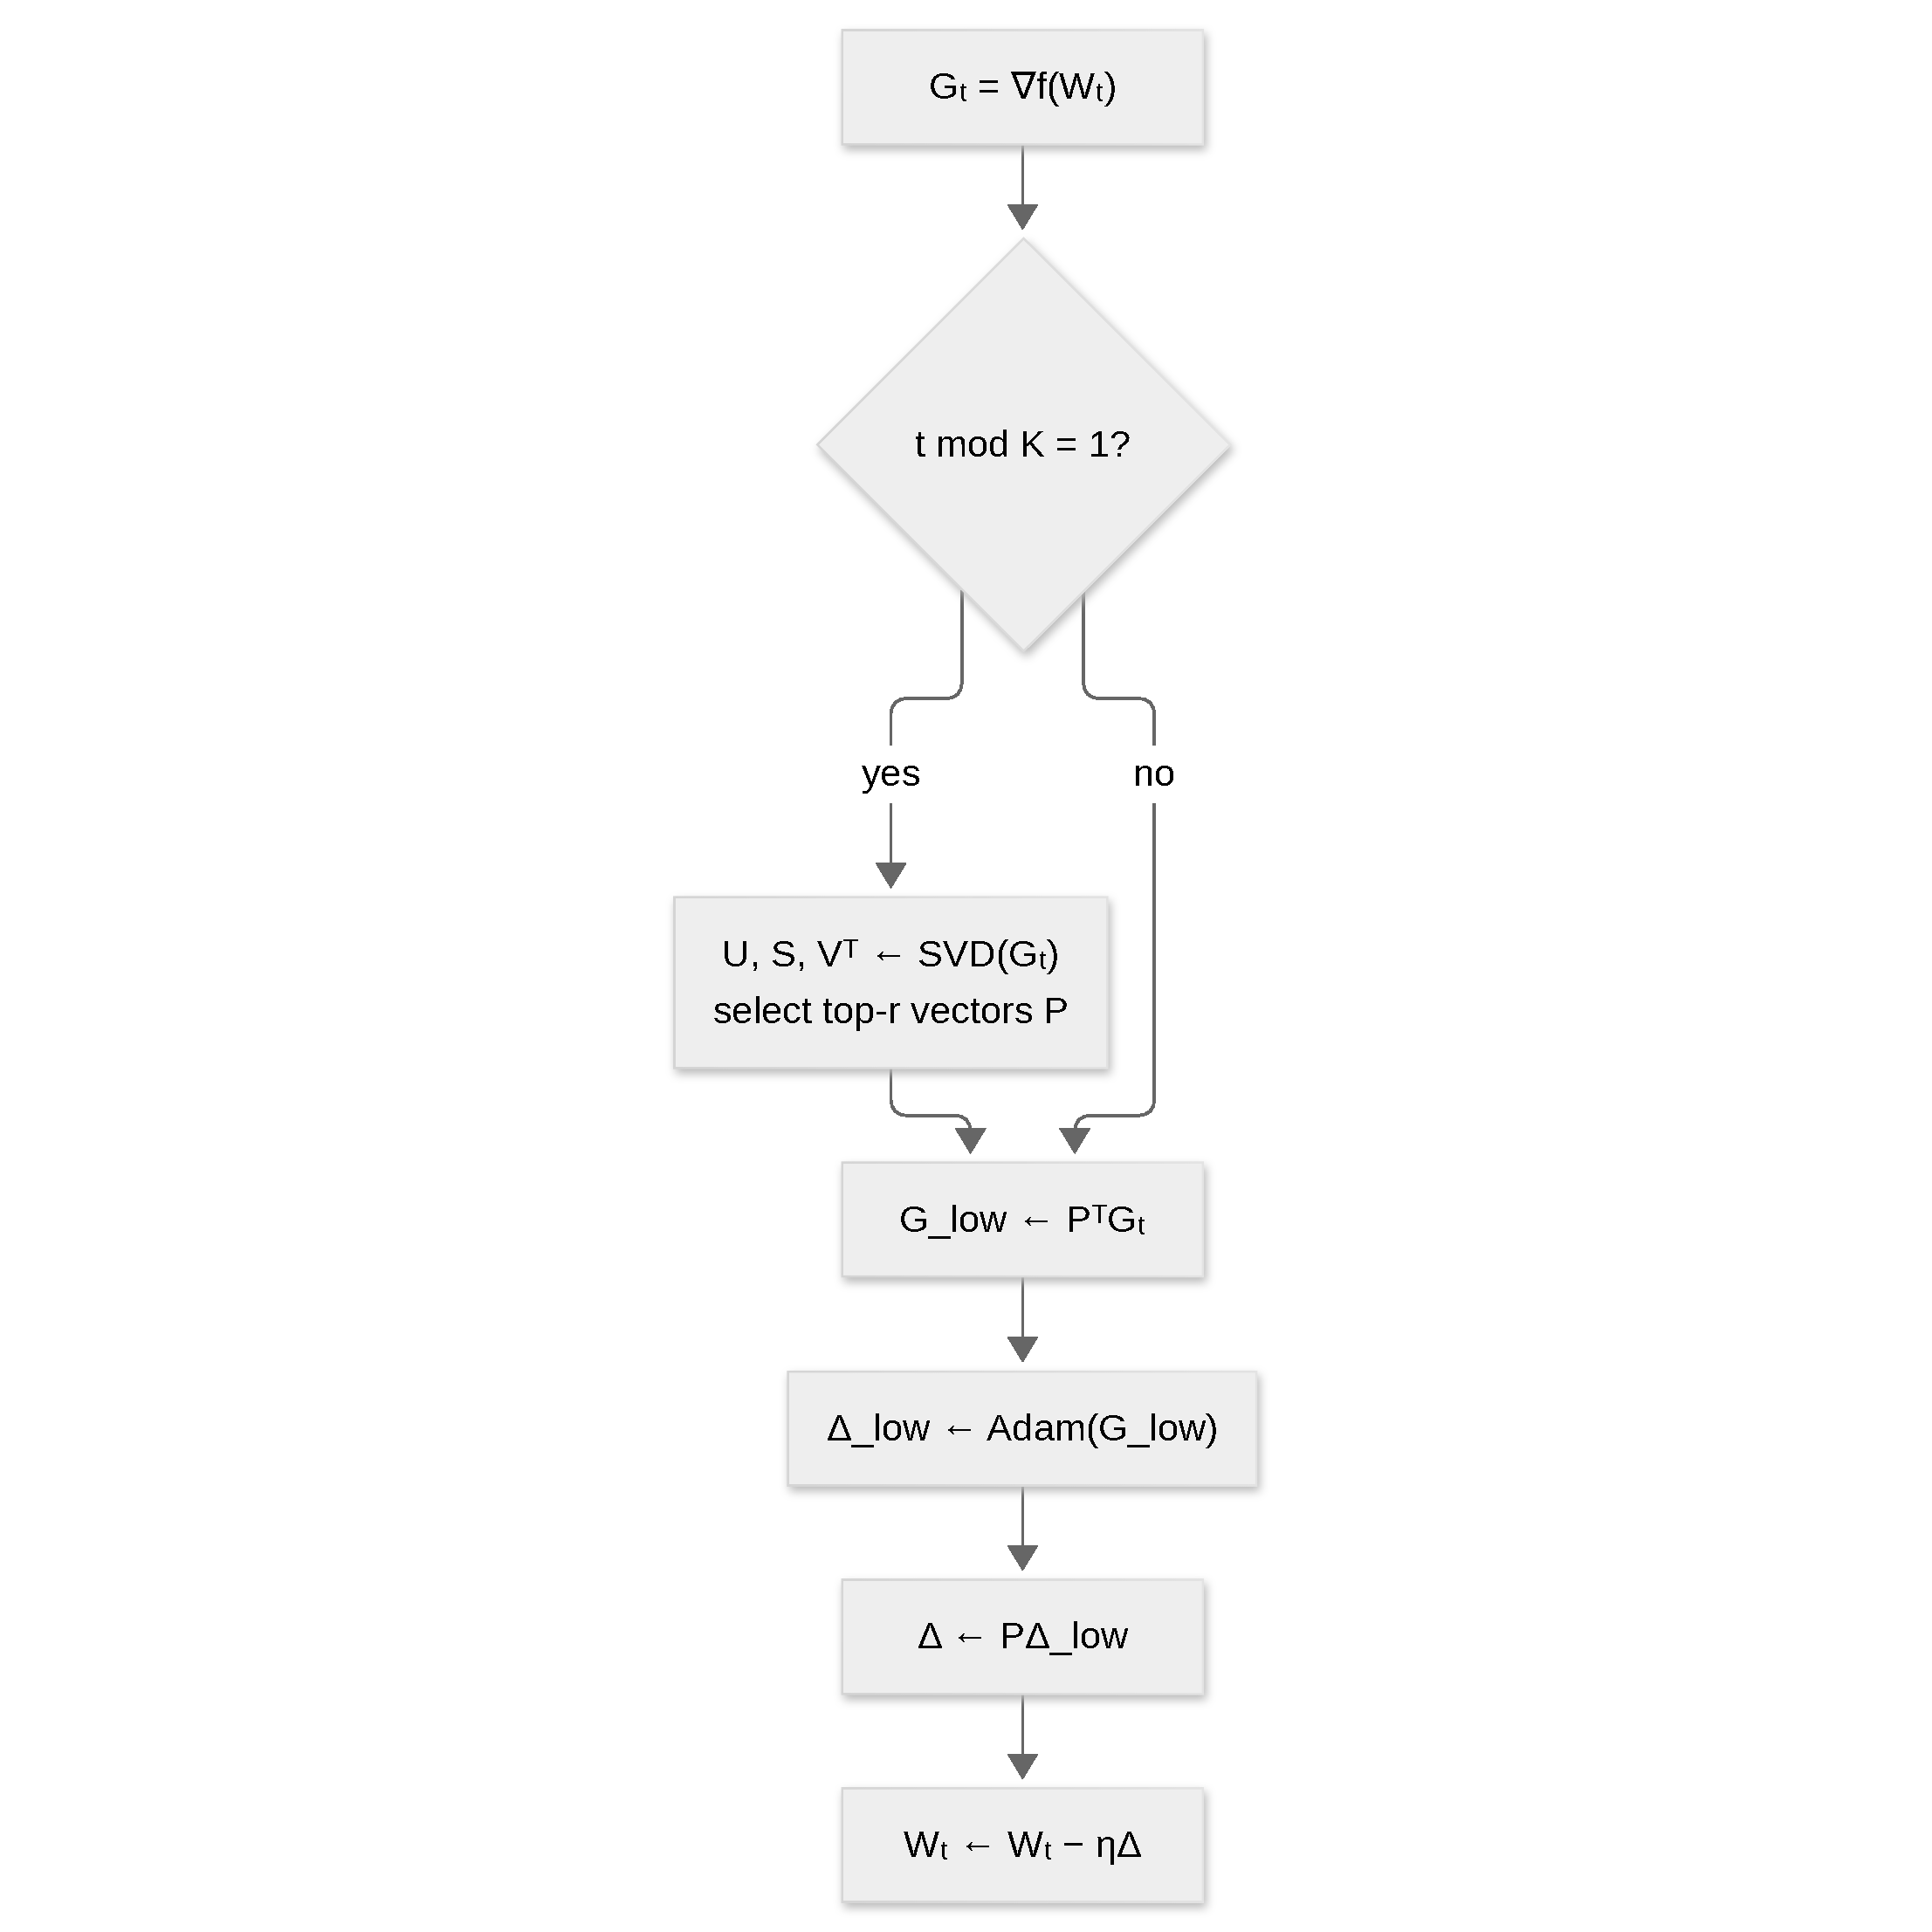
\includegraphics{figures/optimizers/galore.pdf}}
\caption{Step flow of GaLore: periodic SVD projection of the gradient into a low-rank subspace, Adam in that subspace, and reconstruction.}
\label{fig:opt-galore}
\end{figure}
GaLore projects 2D gradients into a low-rank subspace before optimization, reducing optimizer-state memory while maintaining adaptive step scaling. For a 2D parameter matrix $W \in \mathbb{R}^{m \times n}$:
\begin{align}
U, S, V &= \text{SVD}(G_t) \quad\text{(compute singular decomposition)} \\
P &\in \mathbb{R}^{n \times r} \quad\text{or} \quad P^\top \in \mathbb{R}^{r \times m} \quad\text{(select top-$r$ singular vectors)} \\
G_{\text{low}} &= P^\top G_t \quad\text{(project to low-rank space)} \\
\Delta_{\text{low}} &= \text{Adam}(G_{\text{low}}) \quad\text{(optimize in compressed space)} \\
\Delta &= P \Delta_{\text{low}} \quad\text{(reconstruct in original space)}
\end{align}
By projecting into a rank-$r$ subspace (typically $r \ll \min(m,n)$), optimizer state is reduced from $O(mn)$ to $O(r(m+n))$ for 2D parameters. This complementary memory-saving approach is especially relevant when the model is too large for full-rank optimizer state.

\begin{algorithm}[H]
\caption{GaLore (Gradient Low-Rank Projection)}
\label{alg:galore}
\begin{algorithmic}[1]
\Require 2D parameter matrix $W \in \mathbb{R}^{m \times n}$, learning rate $\eta$, rank $r \ll \min(m,n)$
\Ensure Updated parameters $\theta_T$
\State Initialize: Adam state in low-rank space (if rank-2 variant)
\For{$t = 1, 2, \ldots, T$}
    \State $G_t \gets \nabla f(W_t)$
    \If{$t \mod K = 1$}  \Comment{Periodic SVD}
        \State $U_t, S_t, V_t^\top \gets \text{SVD}(G_t)$ (full or thin)
        \State Select projection: $P \gets U_t[:, :r]$ or $P \gets V_t[:, :r]$
    \EndIf
    \State Project gradient: $G_{\text{low}} \gets P^\top G_t$ (or $G_t P^\top$ for right projection)
    \State Run Adam on low-rank: $\Delta_{\text{low}} \gets \text{Adam}(G_{\text{low}})$
    \State Reconstruct in original space: $\Delta \gets P \Delta_{\text{low}}$ (or $\Delta_{\text{low}} P^\top$)
    \State $W_t \gets W_t - \eta \Delta$
\EndFor
\Return $\theta_T$
\end{algorithmic}
\end{algorithm}

\paragraph{Cons.}
\begin{itemize}[leftmargin=*]
\item Periodic SVD adds compute and introduces a projection-refresh interval to tune.
\item Low-rank projection can discard gradient information.
\end{itemize}

\paragraph{Pros.}
\begin{itemize}[leftmargin=*]
\item Optimizer state reduced from $O(mn)$ to $O(r(m+n))$ for 2D parameters.
\item Works synergistically with other techniques and has shown strong results on billion-parameter models.
\end{itemize}

\paragraph{APOLLO, APOLLO-Mini, and Q-APOLLO.}
\begin{figure}[H]
\centering
\fitfigure{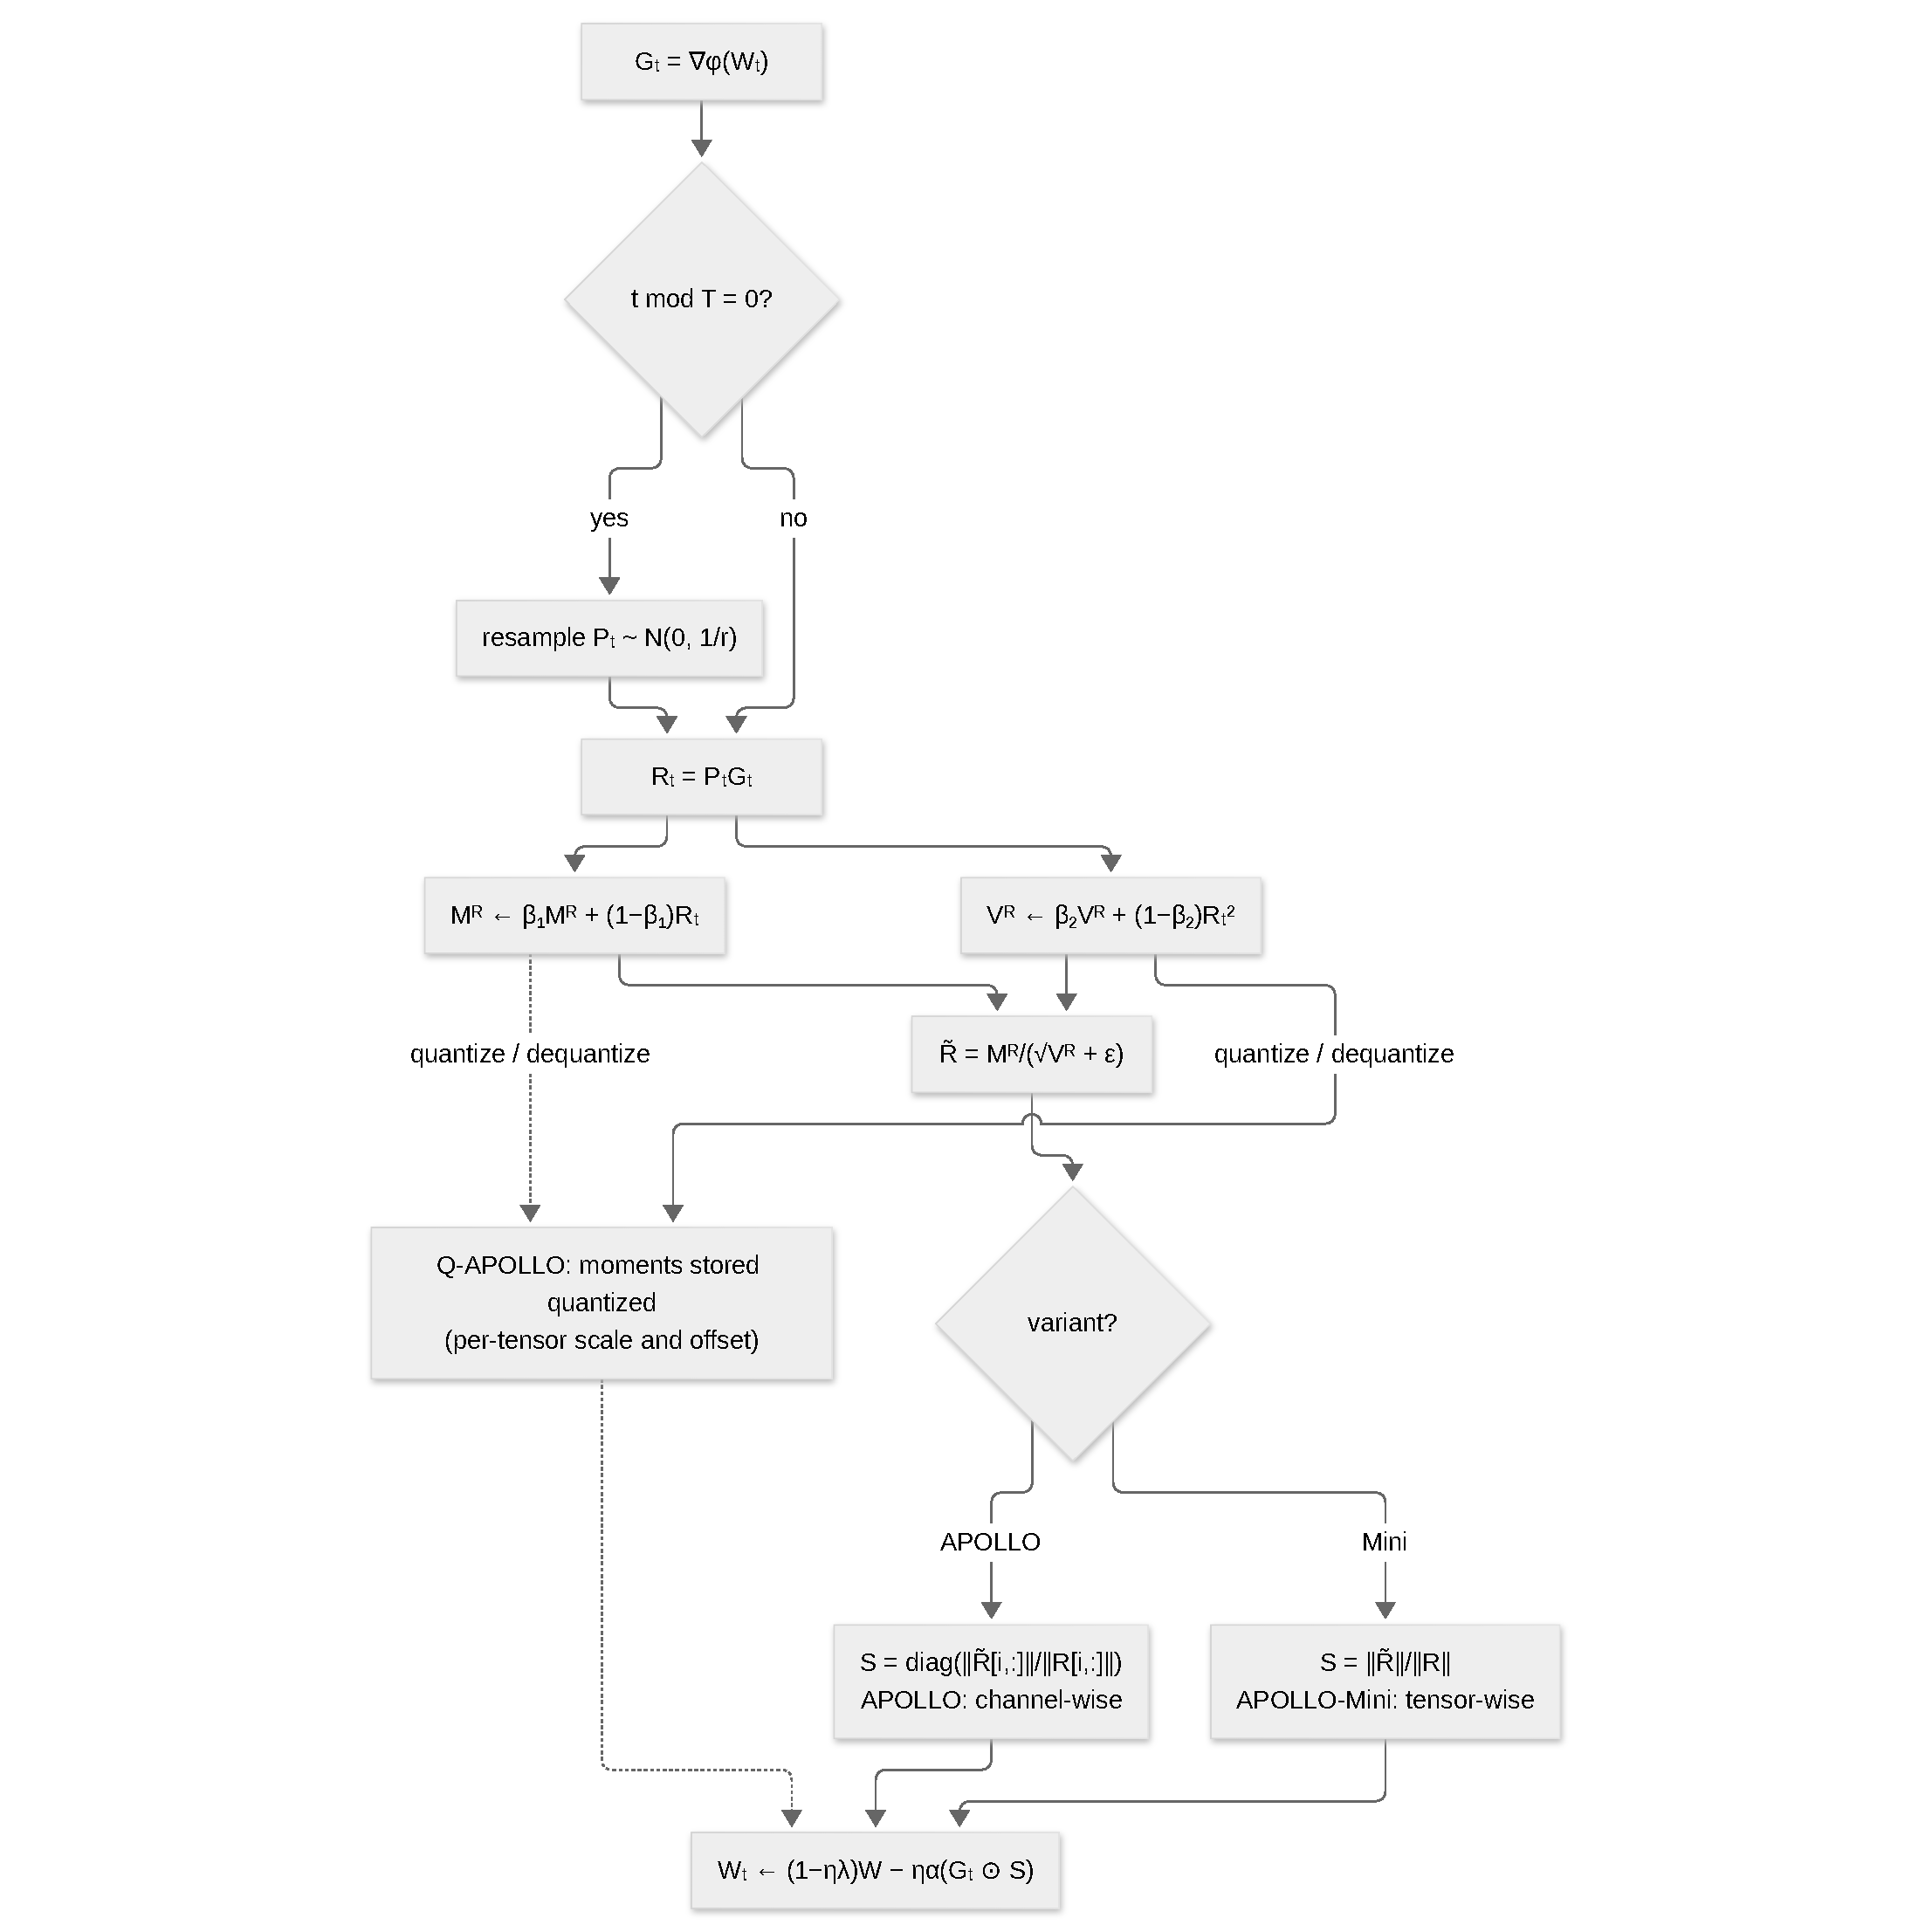
\includegraphics{figures/optimizers/apollo.pdf}}
\caption{Step flow of the APOLLO family: Gaussian-projected moments, structured gradient scaling (channel-wise for APOLLO, scalar for APOLLO-Mini), and quantized state for Q-APOLLO.}
\label{fig:opt-apollo}
\end{figure}
The APOLLO family \citep{zhu2025apollosgdlikememoryadamwlevel} begins from the observation that AdamW's element-wise denominator can be \textbf{coarsened into a structured learning-rate update}. Rather than storing dense moments for every parameter entry, APOLLO projects a matrix gradient $G_t \in \mathbb{R}^{m \times n}$ into a compact random subspace and tracks Adam-style moments there:
\begin{align}
R_t &= P_t G_t \quad\text{or}\quad R_t = G_t P_t^\top \\
M_t^R &= \beta_1 M_{t-1}^R + (1-\beta_1)R_t \\
V_t^R &= \beta_2 V_{t-1}^R + (1-\beta_2)R_t^2 \\
\widetilde{R}_t &= \frac{M_t^R}{\sqrt{V_t^R}+\epsilon}
\end{align}
The projected state is \emph{not} expanded back into a dense low-rank update as in SVD-based methods. Instead, APOLLO estimates a structured scaling tensor $S_t$ in the original space. In the standard APOLLO variant, that scaling is \textbf{channel-wise}: each row or channel receives its own norm ratio. In APOLLO-Mini, the scaling is reduced to a single \textbf{tensor-wise} scalar, corresponding to the rank-1 extreme described in the paper. The resulting parameter update is therefore Adam-like in adaptation but much closer to SGD in state cost:
\[
W_t \gets (1-\eta\lambda)W_{t-1} - \eta\,\alpha\,(G_t \odot S_t)
\]
where $\alpha$ is the extra scale factor used to stabilize highly compressed variants.

\begin{algorithm}[H]
\caption{APOLLO / APOLLO-Mini Structured Gradient Scaling}
\label{alg:apollo-family}
\begin{algorithmic}[1]
\Require Weight matrix $W \in \mathbb{R}^{m \times n}$ with $m \le n$, learning rate $\eta$, scale factor $\alpha$, decay rates $(\beta_1, \beta_2)$, weight decay $\lambda$, rank $r$, projection refresh interval $T$
\Ensure Updated parameters $W_T$
\State Initialize projected moments: $M^R \gets 0$, $V^R \gets 0$, step $t \gets 0$
\Repeat
    \State Compute gradient: $G_t \gets \nabla_W \phi(W_t)$
    \If{$t \bmod T = 0$}
        \State Sample Gaussian projector $P_t \sim \mathcal{N}(0, 1/r)$ with a fresh seed
    \EndIf
    \State Project gradient: $R_t \gets P_t G_t$ \Comment{or $G_t P_t^\top$ depending on layout}
    \State Update projected AdamW moments: $M_t^R, V_t^R \gets \text{AdamWState}(R_t; \beta_1, \beta_2)$
    \State Normalize projected state: $\widetilde{R}_t \gets M_t^R / (\sqrt{V_t^R}+\epsilon)$
    \If{APOLLO}
        \State $S_t \gets \operatorname{diag}(s_1^R, \ldots, s_m^R)$, where $s_i^R = \|\widetilde{R}_t[i,:]\|_2 / \|R_t[i,:]\|_2$
    \Else
        \State $S_t \gets s_t^R$, where $s_t^R = \|\widetilde{R}_t\|_2 / \|R_t\|_2$
    \EndIf
    \State Update weights: $W_t \gets (1-\eta\lambda)W_{t-1} - \eta\,\alpha\,(G_t \odot S_t)$
    \State $t \gets t+1$
\Until{convergence}
\end{algorithmic}
\end{algorithm}

\paragraph{Cons.}
\begin{itemize}[leftmargin=*]
\item Structured scaling is a coarser approximation of AdamW's element-wise denominator.
\item Projectors must be refreshed periodically, and very small ranks make the scaling noisy.
\end{itemize}

\paragraph{Pros.}
\begin{itemize}[leftmargin=*]
\item Replaces repeated SVD with periodically refreshed Gaussian random projection, so the systems cost is ordinary matrix multiplication rather than spectral decomposition.
\item Unusually tolerant to extreme compression: even APOLLO-Mini, which keeps only rank-1 auxiliary state, remains competitive with or better than AdamW while approaching SGD-level memory.
\end{itemize}

\paragraph{APOLLO-Mini.}
APOLLO-Mini is the family member optimized for \textbf{extreme memory efficiency}. The paper motivates it by arguing that, in a rank-1 compact space, channel-wise scaling becomes too noisy, so the update is coarsened further to a single tensor-wise scale. The loss of granularity is partially offset by the explicit scaling factor $\alpha$ (the paper discusses values such as $128$ in this regime), giving a useful point on the optimization Pareto frontier: very small state, no SVD overhead, and still strong pre-training behavior.

\paragraph{Cons.}
\begin{itemize}[leftmargin=*]
\item A single tensor-wise scale loses channel granularity, and rank-1 state can be noisy.
\item Depends on the extra scale factor $\alpha$ (e.g., $128$) to remain stable.
\end{itemize}

\paragraph{Pros.}
\begin{itemize}[leftmargin=*]
\item Smallest state in the APOLLO family, with no SVD overhead.
\item Strong pre-training behavior at near-SGD memory cost.
\end{itemize}

\paragraph{Q-APOLLO.}
The APOLLO paper also stresses that the family combines naturally with \textbf{quantization} for ultra-low-memory training. This repository turns that systems observation into a concrete optimizer variant, \texttt{q\_apollo}. In the implementation, APOLLO's low-rank first and second moments are stored in quantized form together with per-tensor scales and offsets, and are dequantized only when needed for the next step. Q-APOLLO therefore preserves APOLLO's projected-gradient logic while reducing the precision of the remaining optimizer state.

\paragraph{Cons.}
\begin{itemize}[leftmargin=*]
\item Quantized moments introduce approximation error and dequantization overhead.
\item Requires managing per-tensor scales and offsets.
\end{itemize}

\paragraph{Pros.}
\begin{itemize}[leftmargin=*]
\item Reduces the remaining optimizer state to ultra-low precision.
\item Most aggressive memory-saving member of the local optimizer stack while preserving APOLLO's projected-gradient logic.
\end{itemize}

\paragraph{AdamPM (Pooled-Moment Adam).}
AdamPM~\citep{ji_adampm_2026} is a \textbf{minimal, model-agnostic modification of
Adam}: it keeps the element-wise first moment untouched and compresses only the
second moment by \textbf{group-mean pooling of adjacent entries} along each row
(the default, rows being output features) or each column (the paper's
\emph{AdamPM-col}). For a weight matrix $W \in \mathbb{R}^{m \times n}$ and group
size $s$, every row is partitioned into $q = \lceil n/s \rceil$ groups, the
squared gradient is averaged within each group \emph{before} the exponential
moving average, and only the compressed statistic
$\bar{V}_t \in \mathbb{R}^{m \times q}$ is persisted:
\begin{align}
M_t &= \beta_1 M_{t-1} + (1-\beta_1)\, G_t
     && \text{(first moment, element-wise, Eq.~1)} \\
\bar{S}_t &= \frac{1}{s}\sum_{k=1}^{s}
     \mathrm{reshape}(G_t \odot G_t,\, m, q, s)[:,:,k]
     && \text{(within-group means, Eq.~2)} \\
\bar{V}_t &= \beta_2 \bar{V}_{t-1} + (1-\beta_2)\, \bar{S}_t
     && \text{(compressed second-moment EMA, Eq.~3)} \\
W_t &= W_{t-1} - \eta_t \,
     \frac{M_t/(1-\beta_1^t)}
          {\sqrt{\hat{\bar{V}}_t \otimes \mathbf{1}_{1\times s}} + \epsilon},
\qquad \hat{\bar{V}}_t = \frac{\bar{V}_t}{1-\beta_2^t}
     && \text{(update, Eq.~4)}
\end{align}
When $n$ is not divisible by $s$ the final group is padded with its own mean, so
its statistic averages only the entries it actually contains; $s{=}1$ recovers
Adam exactly, and $s \ge n$ collapses each row (or column) to one scalar, the
paper's \emph{AdamPM-inf} limit. AdamPM pools the second moments of
\textbf{all} weight matrices---embeddings, the LM head, attention and MLP
weights---and treats one-dimensional parameters such as RMSNorm scales as
single-row or single-column matrices, so no parameter group is left on a
fallback path. The persistent state is $mn(1+1/s)$ elements against Adam's
$2mn$.

\begin{algorithm}[H]
\caption{AdamPM (Pooled-Moment Adam)}
\label{alg:adampm}
\begin{algorithmic}[1]
\Require Initial parameters $W_0 \in \mathbb{R}^{m\times n}$, steps $T$, group size $s$, learning rate $\eta_t$, decay rates $\beta_1, \beta_2$, stability constant $\epsilon$
\Ensure Updated parameters $W_T$
\State $t \gets 0$; \ $q \gets \lceil n/s \rceil$ \Comment{Number of groups per row}
\State $M_0 \gets \mathbf{0}_{m\times n}$; \ $\bar{V}_0 \gets \mathbf{0}_{m\times q}$ \Comment{First moment and compressed second moment}
\Repeat
    \State $t \gets t + 1$
    \State $G_t \gets \nabla_W \mathcal{L}(W_{t-1})$ \Comment{Gradient}
    \State $M_t \gets \beta_1 M_{t-1} + (1-\beta_1) G_t$ \Comment{First-moment EMA (Eq.~1)}
    \State $\bar{S}_t \gets \operatorname{mean}_{k}\big(\mathrm{reshape}(G_t \odot G_t, m, q, s)[:,:,k]\big)$ \Comment{Group means (Eq.~2)}
    \State $\bar{V}_t \gets \beta_2 \bar{V}_{t-1} + (1-\beta_2) \bar{S}_t$ \Comment{Compressed second-moment EMA (Eq.~3)}
    \State $\hat{M}_t \gets M_t/(1-\beta_1^t)$; \ $\hat{\bar{V}}_t \gets \bar{V}_t/(1-\beta_2^t)$ \Comment{Bias corrections}
    \State broadcast $\hat{\bar{V}}_t$ over each group \Comment{Kronecker product with $\mathbf{1}_{1\times s}$}
    \State $W_t \gets W_{t-1} - \eta_t \hat{M}_t / (\sqrt{\hat{\bar{V}}_t} + \epsilon)$ \Comment{Update (Eq.~4)}
\Until{$t = T$ or convergence}
\Return $W_t$
\end{algorithmic}
\end{algorithm}

Empirically, AdamPM matches a carefully tuned Adam on LLaMA pre-training from
60M to 1.3B parameters while cutting second-moment memory by 87.5\% ($s{=}8$)
to 93.75\% ($s{=}16$), with the same pattern on GLUE fine-tuning of RoBERTa-base
and on TinyLLaVA-1B supervised fine-tuning; group sizes between 2 and 8 are
reported as robust, and three or five---not only powers of two---work because
the incomplete final group is averaged over its own entries.
Theorem~3.1 gives a stationarity bound independent of the group size $s$, and
under a relative-noise condition AdamPM attains the same
$\mathcal{O}(\log T/\sqrt{T})$ rate as Adam. Algorithm~1 of the paper defines no
weight decay; this implementation applies the repository's decoupled
\texttt{wd\_*} decay before the adaptive update, and the shared per-group
\texttt{betas}/\texttt{eps} suffixes parameterize the bias corrections and the
denominator.

\paragraph{Cons.}
\begin{itemize}[leftmargin=*]
\item The diagonal preconditioner becomes coarser as $s$ grows; the paper's
      AdamPM-inf limit shows a measurable perplexity loss at 350M and 1.3B.
\item The saving covers optimizer state only: the first moment stays full-size,
      so optimizer memory is $1+1/s$ of Adam's, not $1/s$.
\item Pooling is one-dimensional (rows or columns); two-dimensional groups and
      selective per-layer pooling remain unexplored (paper limitations).
\end{itemize}

\paragraph{Pros.}
\begin{itemize}[leftmargin=*]
\item Roughly halves optimizer-state memory at the default $s{=}8$ (second
      moment at $1/8$) with Adam-level perplexity through 1.3B parameters and
      negligible per-step overhead---no SVD, no projection, no extra state.
\item Inherits Adam's learning rate and decay rates directly, so existing Adam
      presets transfer without retuning and $\beta_1{=}0.9$, $\beta_2{=}0.95$
      match the repository defaults.
\item Model-agnostic and applies uniformly to every parameter group; the
      preconditioned updates grow more similar to Adam's as model scale grows.
\end{itemize}

\paragraph{Anon (Adaptivity Non-restricted Optimizer with Novel convergence technique).}
\begin{figure}[H]
\centering
\fitfigure{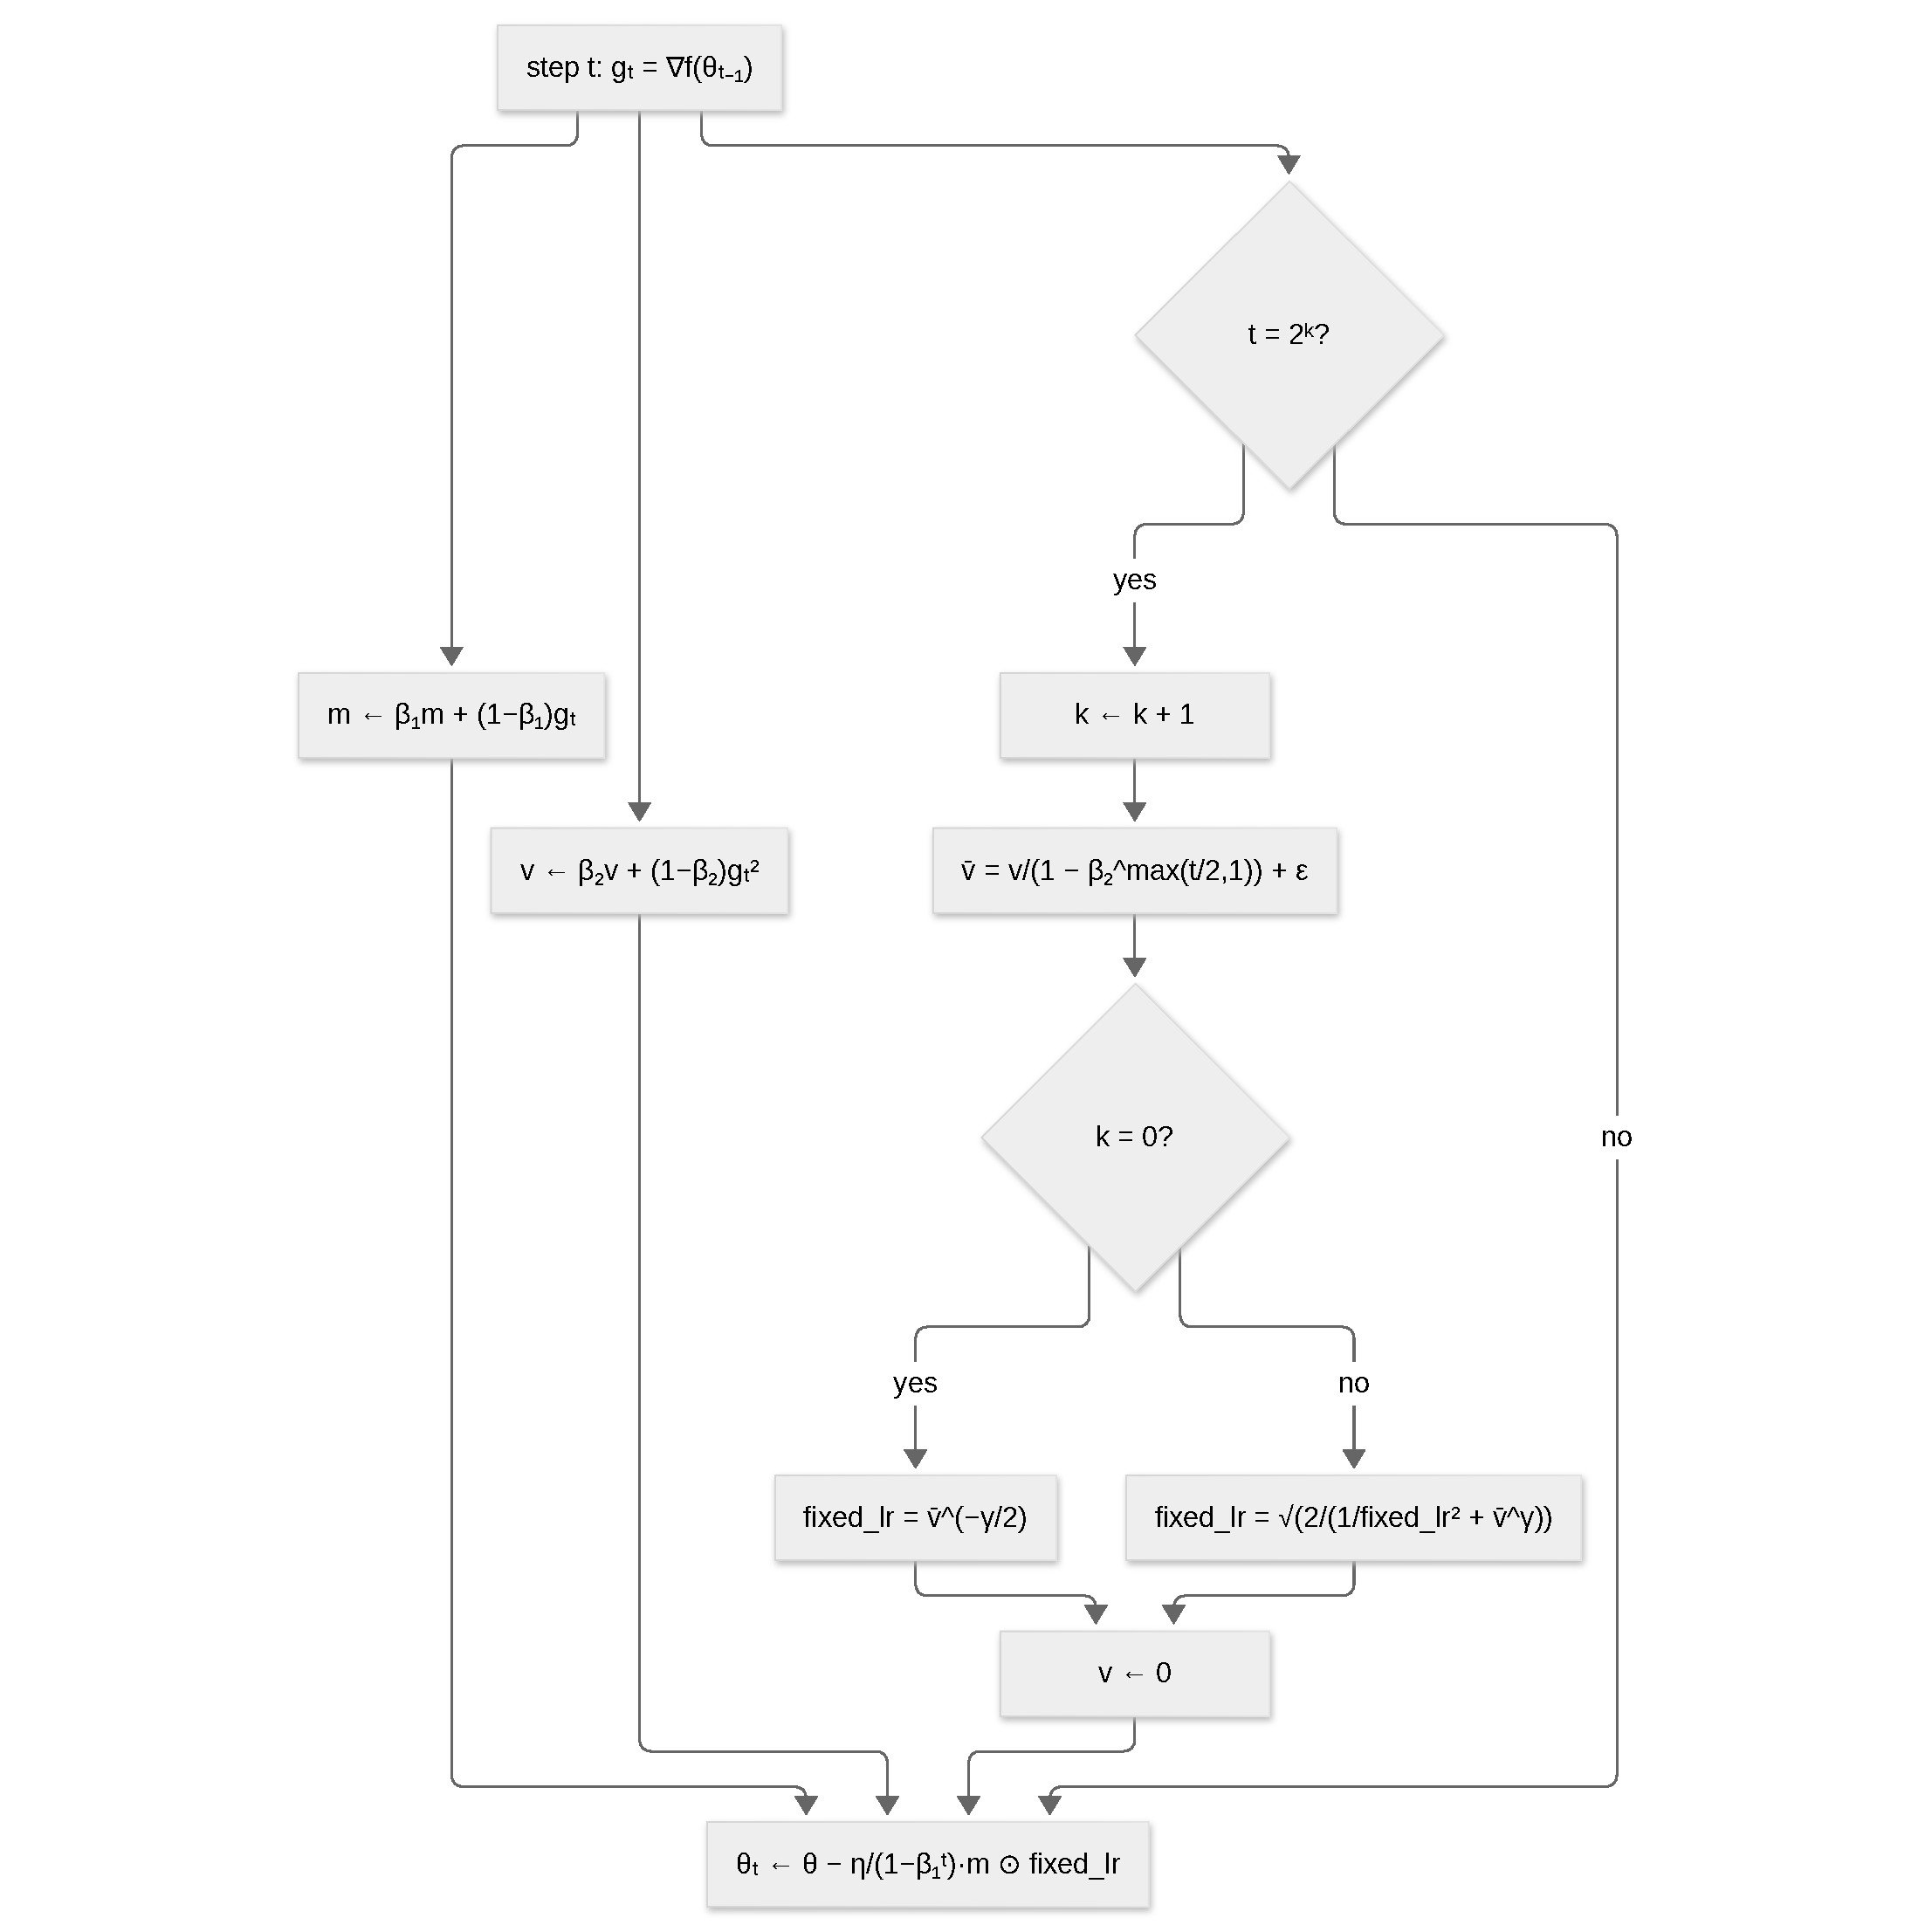
\includegraphics{figures/optimizers/anon.pdf}}
\caption{Step flow of Anon: the IDU preconditioner refreshed at powers of two, with tunable adaptivity $\gamma$ and a bias-corrected momentum update.}
\label{fig:opt-anon}
\end{figure}
Anon \citep{anon2026anon} introduces continuously tunable adaptivity via a single parameter $\gamma \in \mathbb{R}$, bridging the gap between SGD-like ($\gamma=0$) and Adam-like ($\gamma=1$) behaviors, and extrapolating beyond both. The core innovation is the Incremental Delay Update (IDU) mechanism, which enables stable convergence across the entire real-valued adaptivity spectrum:

\begin{align}
m_t &= \beta_1 m_{t-1} + (1-\beta_1) g_t \quad\text{(first moment)}\\
v_t &= \beta_2 v_{t-1} + (1-\beta_2) g_t^2 \quad\text{(second moment)}\\
\bar{v}_t &= \frac{v_t}{1-\beta_2^{\max(t,1)}} + \epsilon \quad\text{(bias-corrected second moment)}\\
\text{fixed\_lr}_k &= \begin{cases}
\bar{v}_k^{-\gamma/2} & \text{if } k = 0 \\
\sqrt{2 / \left(\frac{1}{\text{fixed\_lr}_{k-1}^2} + \bar{v}_k^\gamma\right)} & \text{if } k > 0
\end{cases}\\
\theta_{t+1} &= \theta_t - \frac{\eta}{1-\beta_1^t} \cdot m_t \odot \text{fixed\_lr}_{\lfloor\log_2 t\rfloor}
\end{align}

Unlike standard adaptive optimizers, IDU updates the preconditioner only at powers of two ($t = 2^k$), accumulating gradient statistics between updates and aggregating them recursively. This soft, multi-scale accumulator avoids the hard max-tracking of AMSGrad while provably stabilizing convergence for any $\gamma \in \mathbb{R}$. The parameter $\gamma$ directly controls adaptivity: $\gamma > 1$ accelerates escape from saddle points (favorable for complex architectures), $\gamma = 1$ recovers Adam-like behavior, $\gamma = 0$ yields SGD-like scaling, and $\gamma < 0$ biases toward flatter minima (beneficial for classical architectures like CNNs).

\begin{algorithm}[H]
\caption{Anon (Adaptivity Non-restricted Optimizer with IDU)}
\label{alg:anon}
\begin{algorithmic}[1]
\Require Initial parameters $\theta_0$, learning rate $\eta$, $\beta_1, \beta_2$, tolerance $\epsilon$, adaptivity $\gamma \in \mathbb{R}$
\Ensure Updated parameters $\theta_T$
\State Initialize: $m \gets 0$, $v \gets 0$, fixed\_lr $\gets 0$, step $t \gets 0$, IDU counter $k \gets -1$
\For{$t = 1, 2, \ldots, T$}
    \State $g_t \gets \nabla f(\theta_{t-1})$
    \State $m \gets \beta_1 m + (1-\beta_1) g_t$
    \State $v \gets \beta_2 v + (1-\beta_2) g_t^2$
    \If{$t = 2^k$}
        \State $k \gets k+1$
        \State $\bar{v} \gets v/(1 - \beta_2^{\max(t/2,1)}) + \epsilon$
        \If{$k = 0$}
            \State fixed\_lr $\gets \bar{v}^{-\gamma/2}$
        \Else
            \State fixed\_lr $\gets \sqrt{2 / (1/\text{fixed\_lr}^2 + \bar{v}^\gamma)}$
        \EndIf
        \State $v \gets 0$
    \EndIf
    \State $\theta_t \gets \theta_{t-1} - \frac{\eta}{1-\beta_1^t} \cdot m \odot \text{fixed\_lr}$
\EndFor
\Return $\theta_T$
\end{algorithmic}
\end{algorithm}

\paragraph{Cons.}
\begin{itemize}[leftmargin=*]
\item Maintains three state buffers ($m$, $v$, fixed\_lr) and refreshes the preconditioner on a logarithmic schedule.
\item The adaptivity parameter $\gamma$ must be selected per architecture.
\end{itemize}

\paragraph{Pros.}
\begin{itemize}[leftmargin=*]
\item Same $\mathcal{O}(n)$ per-step complexity class as AdamW, with continuously tunable adaptivity.
\item IDU provably attains $\mathcal{O}(\sqrt{T})$ regret for convex problems and $\mathcal{O}(\ln T / \sqrt{T})$ for non-convex settings.
\end{itemize}

\paragraph{Prodigy (Approximating the Distance Estimate).}
\begin{figure}[H]
\centering
\fitfigure{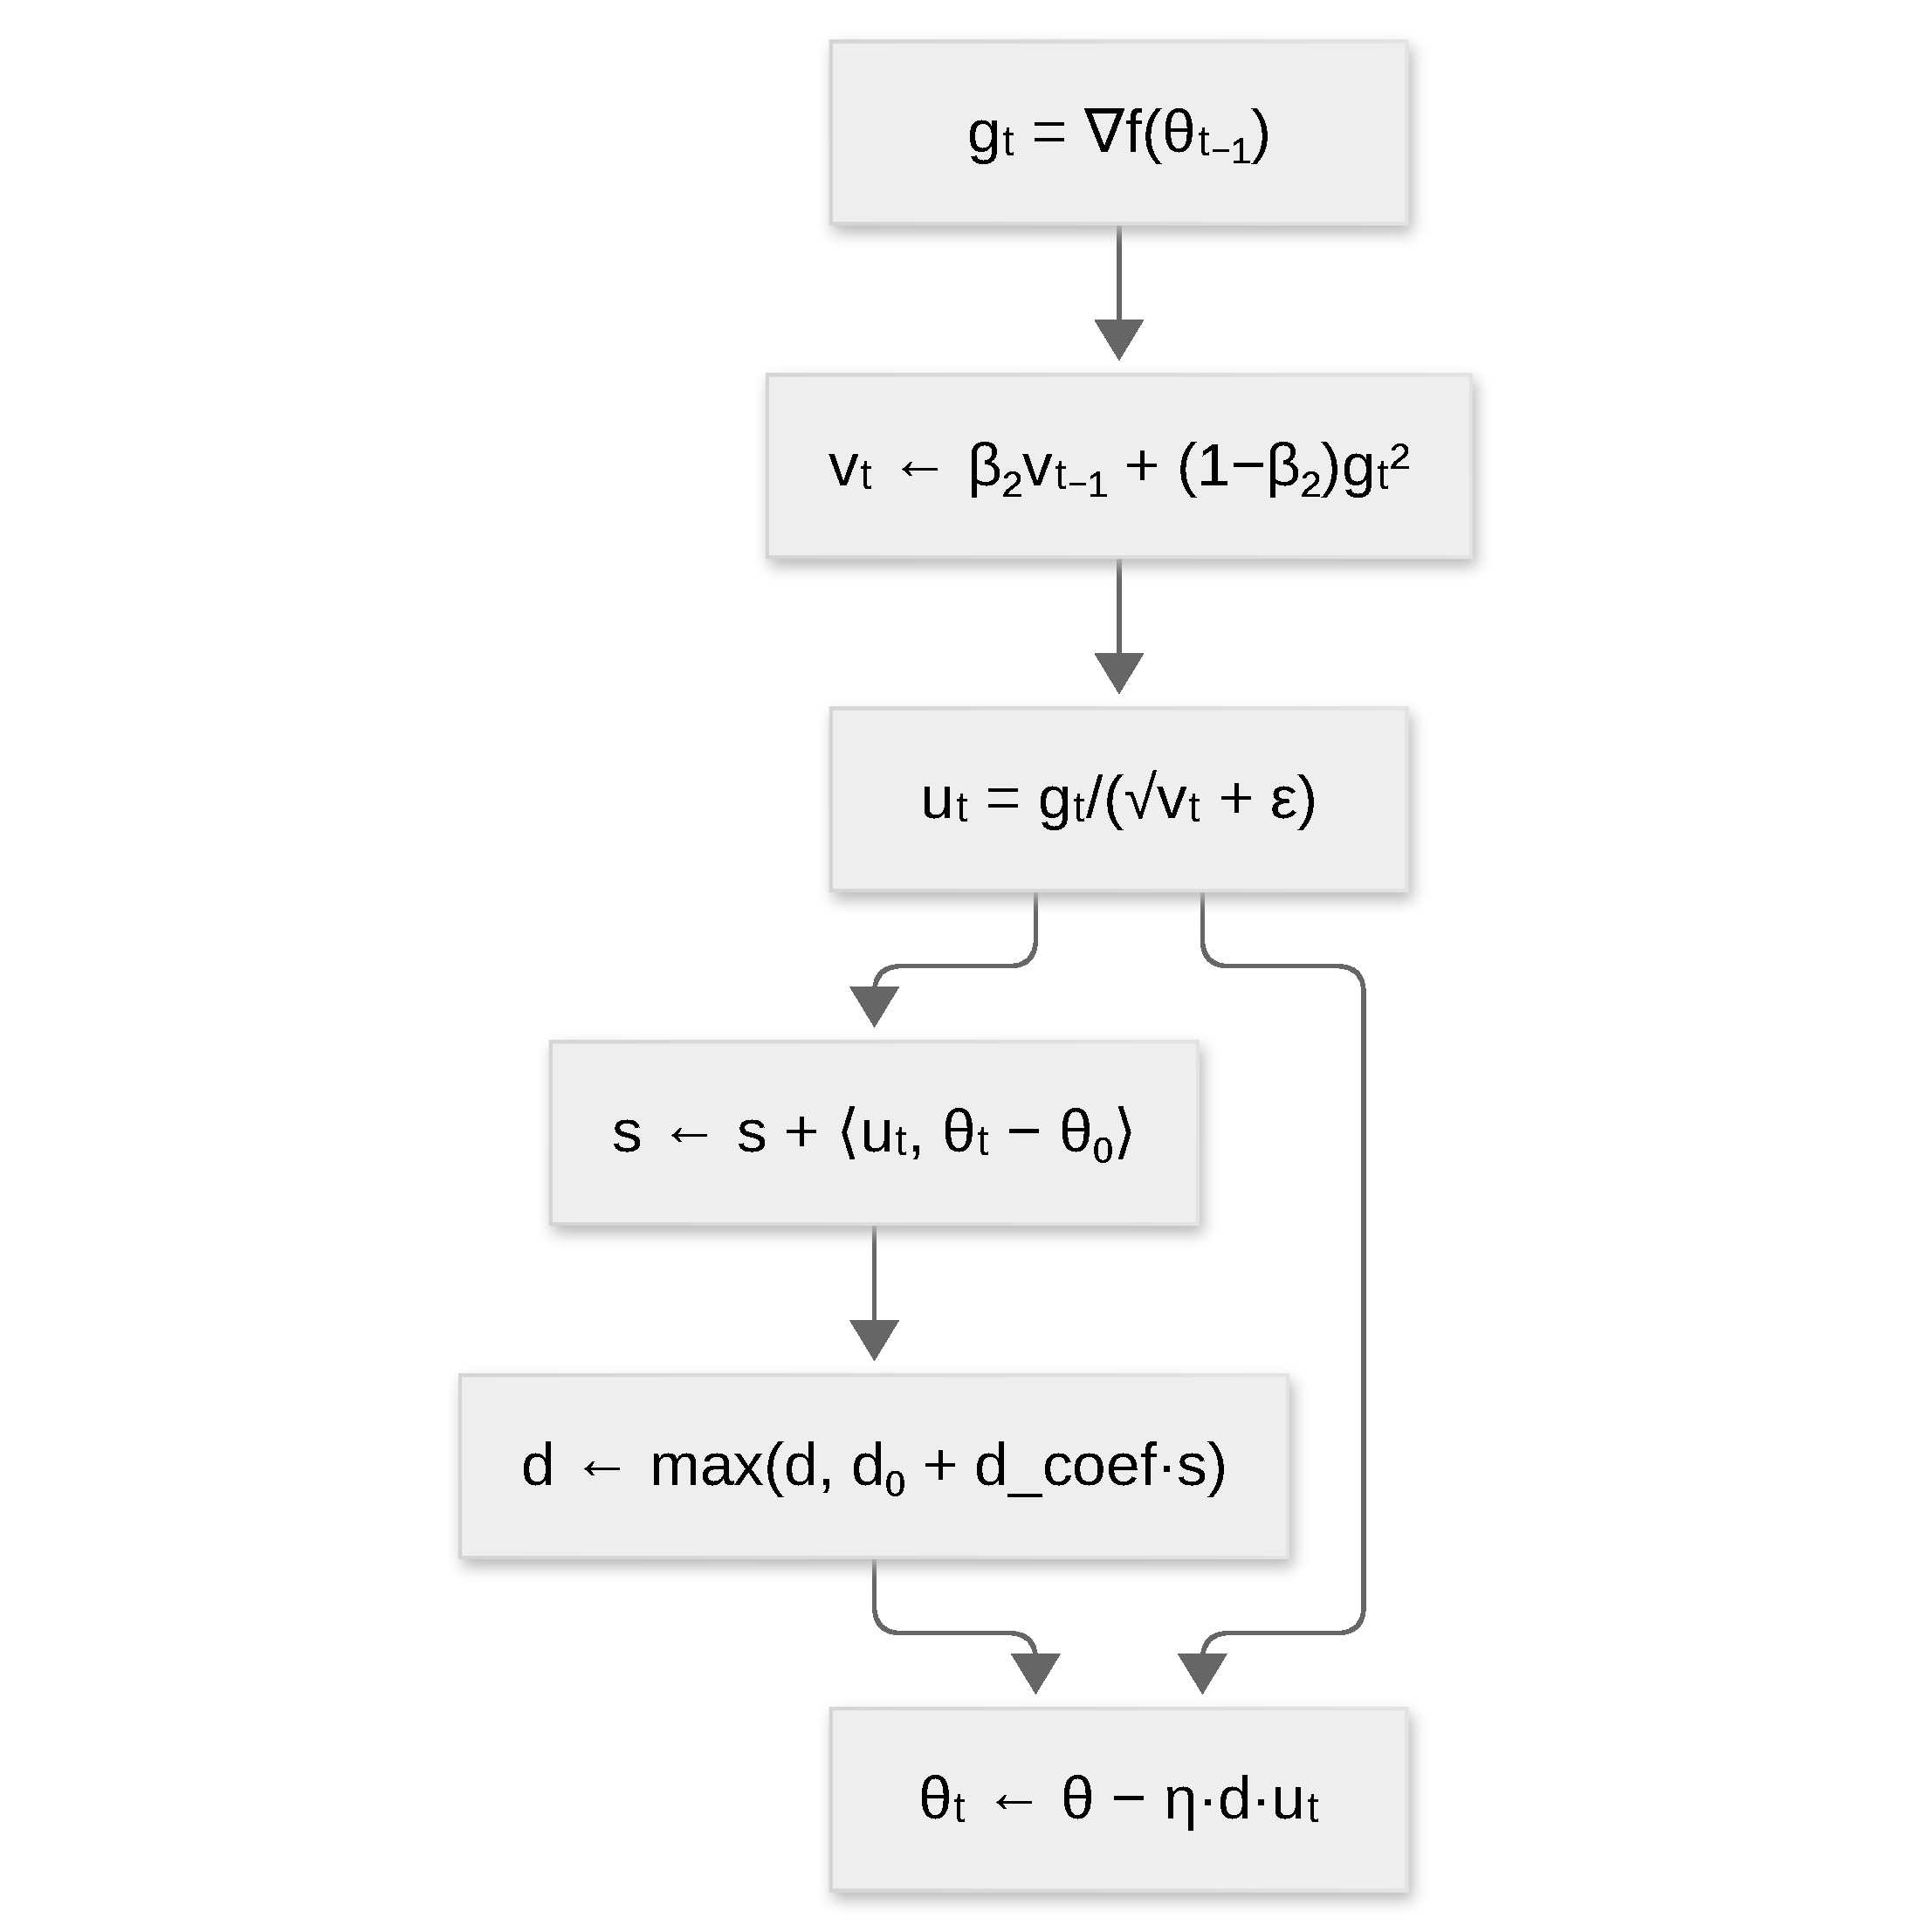
\includegraphics{figures/optimizers/prodigy.pdf}}
\caption{Step flow of Prodigy: a cumulative signed-distance estimate that scales the adaptive step without a learning-rate schedule.}
\label{fig:opt-prodigy}
\end{figure}
Prodigy adapts the effective step scale through a running distance-like statistic, eliminating the need for explicit learning-rate tuning. The algorithm maintains a cumulative distance estimate:
\begin{align}
u_t &= \frac{g_t}{\sqrt{v_t}+\epsilon} \quad\text{(unnormalized adaptive step)} \\
s_t &= s_{t-1} + \langle u_t, \theta_t - \theta_0 \rangle \quad\text{(cumulative signed distance)} \\
d_t &= \max(d_{t-1}, d_0 + d_{\text{coef}} \cdot s_t) \quad\text{(distance estimate with lower bound)} \\
\theta_{t+1} &= \theta_t - \eta \cdot d_t \cdot u_t
\end{align}
where $d_0$ is an initial bound and $d_{\text{coef}}$ controls how aggressively the estimate adapts. The distance estimate $d_t$ captures the combined magnitude of past gradients weighted by actual parameter displacement, implementing an implicit effective learning rate.

\begin{algorithm}[H]
\caption{Prodigy (Approximating the Distance Estimate)}
\label{alg:prodigy}
\begin{algorithmic}[1]
\Require Initial parameters $\theta_0$, learning rate $\eta$, coeff $d_{\text{coef}}$, initial dist $d_0 > 0$
\Ensure Updated parameters $\theta_T$
\State Initialize: $s \gets 0$ (cumulative signed distance), $d \gets d_0$
\For{$t = 1, 2, \ldots, T$}
    \State $g_t \gets \nabla f(\theta_{t-1})$
    \State $v_t \gets \beta_2 v_{t-1} + (1-\beta_2) g_t^2$ \Comment{Second moment}
    \State $u_t \gets g_t / (\sqrt{v_t} + \epsilon)$ \Comment{Unnormalized adaptive}
    \State Update distance: $s \gets s + \langle u_t, \theta_t - \theta_0 \rangle$ \Comment{Signed distance}
    \State $d \gets \max(d, d_0 + d_{\text{coef}} \cdot s)$ \Comment{Lower-bounded distance}
    \State $\theta_t \gets \theta_{t-1} - \eta \cdot d \cdot u_t$ \Comment{Distance-scaled update}
\EndFor
\Return $\theta_T$
\end{algorithmic}
\end{algorithm}

\paragraph{Cons.}
\begin{itemize}[leftmargin=*]
\item Introduces $d_0$ and $d_{\text{coef}}$ hyperparameters for the distance estimate.
\item Adds an inner-product bookkeeping step per iteration.
\end{itemize}

\paragraph{Pros.}
\begin{itemize}[leftmargin=*]
\item Removes explicit learning-rate tuning and scheduling.
\item Robust convergence across problem scales and batch sizes.
\end{itemize}

